
%%% Local Variables:
%%% mode: latex
%%% TeX-master: t
%%% End:

\documentclass[12pt,a4paper,ngerman]{article}
\usepackage{microtype}
\usepackage{ae}
\usepackage[utf8x]{inputenc}
\usepackage[T1]{fontenc}
\usepackage{t1enc}
\usepackage{type1cm}
\usepackage[main=german,ngerman]{babel}
\usepackage{graphicx}

\usepackage{ifpdf}
\ifpdf
\usepackage{xmpincl}
\usepackage[pdftex]{hyperref}
\hypersetup{
    colorlinks,
    citecolor=black,
    filecolor=black,
    linkcolor=black,
    urlcolor=black,
    bookmarksopen=true,     % Gliederung öffnen im AR
    bookmarksnumbered=true, % Kapitel-Nummerierung im Inhaltsverzeichniss anzeigen
    bookmarksopenlevel=1,   % Tiefe der geöffneten Gliederung für den AR
    pdfstartview=FitV,       % Fit, FitH=breite, FitV=hoehe, FitBH
    pdfpagemode=UseOutlines, % FullScreen, UseNone, UseOutlines, UseThumbs 
}
\pdfinfo{
  /Author (Eckhart Arnold)
  /Title (Kann die evolutionaere Spieltheorie die Entstehung von Kooperation erklaeren? Studie ueber die Schwaechen eines formalen Ansatzes)
  /Subject (Eine Kritik evolutionaerer Computersimulationen zur Erklaerung der Entstehung von Kooperation)
  /Keywords (Evolutionaere Spieltheorie, Formale Methoden in den Sozialwissenschaften, Evolution der Kooperation, Simulation des Gesellschaftsvertrags)
}
\includexmp{Kritik_der_Spieltheorie}
\fi

%\usepackage{fancyhdr}
%\pagestyle{fancy}
%\pagestyle{myheadings}

%\setlength{\headheight}{15pt}
%\addtolength{\headheight}{\baselineskip}

%\fancyfoot{}

%\renewcommand{\chaptermark}[1]{\markboth{\chaptername \ \thechapter.\ #1}{}}
%\renewcommand{\chaptermark}[1]{\markboth{#1}{}}
%\renewcommand{\sectionmark}[1]{\markright{\thesection.\ #1}}

%\renewcommand{\headrulewidth}{0.4pt}
%\renewcommand{\footrulewidth}{0pt}

%\addtolength{\textwidth}{-1cm}
%\addtolength{\headwidth}{\marginparsep}
%\addtolength{\headwidth}{\marginparwidth}

%\setlength{\oddsidemargin}{0cm}
%\setlength{\evensidemargin}{0cm}

\sloppy

\setcounter{page}{1}

\begin{document}
\selectlanguage{\ngerman}

\title{Kann die evolutionäre Spieltheorie die Entstehung von Kooperation erklären?\\Studie über die Schwächen eines formalen Ansatzes}
\author{Eckhart Arnold}
\date{25.5.2005}
\maketitle
\begin{abstract}

  Computer models of evolutionary game theory have in the last 20 or
  30 years been widely used to study such phenomena as cooperation and
  reciprocal altruism. However, the scientic value of these models
  remains often rather doubtful. In this paper I try to demonstrate
  (by examining several examples) that these models are often indeed
  empirically imprecise and theoretically shallow. Furthermore, I try
  to answer why these models often fail and, finally, what
  requirements a model must meet if it is to be of any explanatory
  relevance.

\end{abstract}

\newpage

\pagenumbering{roman}
\tableofcontents

\newpage

\setcounter{page}{1}
\pagenumbering{arabic}

\section{Einleitung}

Die evolutionäre Spieltheorie erfreut sich seit etwa 30 Jahren größter
Beliebtheit. Ursprünglich von Biologen entwickelt um strategische
Aspekte der Evolution, wie z.B. häufigkeitsabhängige Selektion, zu
beschreiben, wird sie heute als Teildisziplin der Spieltheorie in den
unterschiedlichsten Fachbereichen (Biologie, Ökonomie, Soziologie,
Politische Wissenschaften) angewendet. Erheblichen Auftrieb erhielt
die evolutionäre Spieltheorie vor allem durch die Veröffentlichungen
von Maynard-Smith und Robert Axelrod anfang der 80er Jahre. Besonders
Axelrod trug durch den innovativen Gebrauch von Computersimulationen
und durch die Breite seiner Anwendungsbeispiele wesentlich dazu bei,
die evolutionäre Spieltheorie als wissenschaftlichen Ansatz in den
unterschiedlichsten Fachbereichen zu popularisieren. Große Hoffnungen
verbanden sich mit diesem neuartigen Ansatz. Indem nämlich die
evolutionäre Spieltheorie nicht an die strikten "`rational choice"'
Annahmen gebunden ist, durch die manche Gedankengänge der
konventionellen Spieltheorie oft so überaus artifiziell
erscheinen,\footnote{Ein Beispiel ist das Argument der
  Rückwärtsinduktion, das für das endlich oft wiederholte
  Gefangenendilemma den Zusammenbruch von Kooperation vorhersagt. Das
  Argument der Rückwärtsinduktion trifft nur unter der Voraussetzung
  unbedingter wechselseitiger Rationalität zu. Ein evolutionäres
  System konvergiert nur extrem langsam zu dieser Lösung, und auch der
  experimentellen Befund steht mit dem Argument nicht im Einklang.}
konnte man erwarten, dass die evolutionäre Spieltheorie als
verfeinerte und flexiblere Form der Spieltheorie neue
Anwendungsbereiche erschließen würde; darunter womöglich auch solche,
die einer formal exakten Theoriebildung bisher überhaupt verschlossen
geblieben waren. Letzteres schien umso mehr zu gelten als der Einsatz
von Computertechnik, die sich zur selben Zeit rasch entwickelte, die
formale Modellbildung sowohl stark vereinfacht als auch ihre
Leistungsfähigkeit drastisch erhöht.

Haben sich diese teils recht hochgespannten Erwartungen inzwischen
erfüllt? Dass neuartige Ansätze immer auch Kritik auf den Plan rufen,
ist an sich nichts Ungewöhnliches \cite{alexander:2003}. Aber während
es in den frühen Tagen der evolutionären Spieltheorie noch anging,
berechtigte Kritik durch den Hinweis zu entkräften, dass es sich eben
um eine noch junge Disziplin handele \cite[S. 38]{schuessler:1997}, die
noch weiterentwickelt werden müsse, so können über 20 Jahre später
derartige Entschuldigungen nicht mehr gelten. Es ist vielmehr an der
Zeit, nüchtern Bilanz zu ziehen, was die simulationsgestützte
evolutionäre Spieltheorie bisher hat erreichen können, und welche
Leistungen man von diesem Ansatz in Zukunft noch wird erwarten
dürfen. Um einen Beitrag zu einer solchen Bilanz zu leisten, möchte
ich im Folgenden untersuchen, was die Theorie der Kooperation, wie sie
von Axelrod beschrieben und von zahlreichen Nachahmern und Nachfolgern
verfeinert und ausgebaut worden ist, in Anwendung auf unterschiedliche
Problemstellungen leistet. Hinsichtlich dieser Anwendungsbeispiele,
die vorwiegend dem historisch-politischen Bereich entnommen sind,
fällt meine Bilanz eher sehr skeptisch aus:

\begin{enumerate} 

\item Auch der
evolutionären Spieltheorie gelingt nicht die Urzeugung mathematisch
exakter gesellschaftswissenschaftlicher Theoriebildung. Formale
Modelle werden in den Gesellschaftswissenschaften auch in Zukunft nur
ein marginalisiertes Dasein fristen als (allerdings unerläßliche)
Hilfswissenschaften wie z.B. die Sozialstatistik oder eingebettet in
einen umfassenderen und wesentlich nicht formalen Erklärungskontext.

\item Die Computermodelle der evolutionären Spieltheorie erweisen sich
in hohem Maße als "`explanatorisch irrelevant"' \cite{alexander:2003},
indem ihre Anwendung eine sehr präzise Situationsbeschreibung
voraussetzt, aus der sich die Erklärung der Sitaution oft schon ohne
Modell ergibt.  

\item Nur in Ausnahmenfällen ist eine
Beschreibung der Problemsituation möglich, die so exakt ist, dass sie
es erlaubt, mit einem formalen Modell überhaupt anzusetzen. Erfordert
wird hierfür, dass (1) sämtliche kausal relevanten Einflussgrößen im
Modell erfasst werden, und dass (2) die entsprechenden Parameter genau
genug gemessen werden können, um stabile Vorhersagen durch das Modell
zu ermöglichen. Sind diese Bedingungen, wie es leider häufig der Fall ist,
nicht gegeben, dann schrumpft das Erklärungspotential formaler Modelle
auf das epistemologische Niveau bloßer Metaphern zusammen.  

\item Die
mathematisch-technische Verfeinerung der formalen Modellierung und die
Erprobung immer neuer Varianten von Computersimulationen allein führt
weder zu einer Erweiterung des Anwendungsbereichs der Theorie der
"`Evolution der Kooperation"' noch wird sie durch eine Erhöhung der
Erklärungskraft der Theorie belohnt. Impulse für die Weiterbildung
dieses Ansatzes sind -- wenn überhaupt -- nur von der Empirie zu erwarten.

\end{enumerate} 

Da die Beispiele, auf die sich dieser Befund stützt, sich weitgehend
auf die Theorie der "`Evolution der Kooperation"' beschränken,
berühren sie natürlich nur einen Teilbereich der
evolutionären Spieltheorie, auch wenn zu befürchten ist, dass die
Grundprobleme die evolutionäre Spieltheorie im Ganzen
betreffen, besonders dann wenn sie außerhalb von Biologie und Ökonomie
angewendet wird. In gewisser Weise spiegeln die Schwächen der evolutionären
Spieltheorie dabei nur die Schwierigkeiten wieder, denen Versuche der
exakten Theoriebildung in bestimmten Wissenschaftsbereichen immer
wieder begegnen. 

Nun könnte man einwenden, dass bei den oben angeführten Punkten
Erwartungen an die evolutionäre Spieltheorie gestellt werden, die
höchstens von übermäßig selbstbewussten Vertretern der Disziplin
genährt werden, während in Wirklichkeit eine sehr viel besonnenere
Haltung vorherrscht. Dabei scheint die evolutionäre Spieltheorie aber
in das Dilemma zu geraten, dass sie sich entweder hochgesteckte Ziele
setzen kann, die bis hin zu dem Anspruch reichen, Probleme der
Gesellschaftsvertragstheorie spieltheoretisch erörtern zu wollen,
denen die spieltheoretischen Modelle dann aber nicht ansatzweise
gerecht werden, oder sich bescheiden auf den Standpunkt zurückziehen
kann, dass Modelle eben nur Modelle sind, die keine unmittelbaren
Schlussfolgerungen auf die Wirklichkeit zulassen, was dann
zwangsläufig die Frage aufwirft, wozu die Erforschung von Modellen
eiegentlich gut ist.

Fairerweise muss jedoch eingeräumt werden, dass selbst in
Wissenschaftsbereichen, die in der Regel keine exakte Theoriebildung
zulassen, die evolutionäre Spieltheorie auch Einiges auf der Haben-Seite
zu verbuchen hat: 

\begin{enumerate} 

\item Die (evolutionäre) Spieltheorie 
liefert ein reichhaltiges Reservoir an Metaphern und Modellbeispielen,
die unsere wissenschaftliche Vorstellungskraft und die "`Fantasie für
das Mögliche"' erheblich bereichern.  

\item Insbesondere erlaubt es
die Theorie der "`Evolution der Kooperation"', vereinfachte und
falsche Vorstellungen über die Natur und das Ergebnis evolutionärer
Prozesse, wie z.B. das "`Überleben der Stärkeren"', die Unmöglichkeit
egoistischer Kooperation etc., begründet zurückzuweisen.

\item Die {\em evolutionäre} Spieltheorie leistet einen konstruktiven Beitrag zur
Kritik allzu enger "`rational choice"' Annahmen. Sie trägt, indem sie eine
glaubwürdige Alternative anbietet, zum besseren Verständnis
davon bei, warum sich in vielen Situationen gerade nicht egoistisch-rationales
Verhalten langfristig durchsetzt.

\end{enumerate} 


\section{Die Theorie der "`Evolution der Kooperation"'}

Wenn im folgenden von der Theorie der "`Evolution der Kooperation"'
die Rede ist, dann ist damit vor allem Robert Axelrods Theorie der
"`Evolution der Kooperation"' gemeint, sowie deren Weiterentwicklung
und Modifikation durch andere Autoren wie beispielsweise Rudolf
Schüßler, Bryan Skyrms und andere. Um nun zu zeigen, was diese
Theorie leisten kann und, wichtiger noch, was sie nicht leistet, muss
zunächst einmal die Theorie selbst dargestellt werden. Dazu ist
zu klären:

\begin{enumerate}

\item Was will die Theorie der "`Evolution der Kooperation"' erklären?

\item Wie erklärt sie das, was sie zu erklären beanchsprucht?

\item Welche Alternativ- oder Konkurrenztheorien gibt es?

\end{enumerate}

\subsection{Was die Theorie der "`Evolution der Kooperation"' zu
erklären beansprucht}

Die Frage, was die Theorie der "`Evolution der Kooperation"' zu
erklären beansprucht, ist nicht ganz leicht zu beantworten, da die
verschiedenen Autoren, die zu dieser Theorie beigetragen haben,\footnote{Die
folgenden Ausführungen stützen sich vor allem auf die Darstellungen von Robert
Axelrod \cite{axelrod:1984}, Rudolf Schüßler \cite{schuessler:1997}, Brian
Skyrms \cite{skyrms:1996, skyrms:2004} und Ken Binmore \cite{binmore:1994,
binmore:1998}.} mit unterschiedlichen (und vor allem auch recht unterschiedlich
bescheidenen) Erklärungsansprüchen auftreten.  Summarisch
zusammengefasst kann man dabei grob die drei folgenden Zielsetzungen
ausmachen:

\begin{enumerate}

\item Die Theorie der "`Evolution der Kooperation"' soll eine
{\em Generalerklärung} dafür bereitstellen, warum überhaupt
kooperatives Verhalten in der natürlichen wie in der
kulturellen\footnote{Für den Begriff der kulturellen Evolution, der in
einem darwinistischen Sinne, aber ohne eine strikte Analogie zur
natürlichen, d.h. genetischen Evolution zu postulieren, verstanden
wird vgl.: \cite{schurz:2001}} Evolution entstehen konnte.

\item Zugleich beansprucht sie, Einzelerklärungen für die unterschiedlichsten
Situationen zu liefern, in denen kooperatives Verhalten beobachtet
werden kann.

\item Speziell im Hinblick auf die politische Philosophie und insbesondere die
Gesellschaftsvertragstheorie ist es ein Anliegen der Theorie der
"`Evolution der Kooperation"' zu zeigen, inwiefern Kooperation auch
unter egoistischen Individuen denkbar ist, ohne dass sie durch eine
zentrale Gewalt erzwungen werden muss.

\end{enumerate}

Alle drei Aspekte der Theorie der "`Evolution der Kooperation"' werden
im Rahmen der weiter unten aufgeführten Beispiele zur Sprache
kommen. Zunächst ist zu erörtern, wie die Theorie der "`Evolution der
Kooperation"' vorgeht, um Kooperation zu erklären.


\subsection{Die Gestalt der Erklärungen der Theorie der "`Evolution der
Kooperation"'}

Die Theorie der "`Evolution der Kooperation"' gibt es, wie schon
bemerkt, in vielfältigen Varianten. Den meisten davon ist gemeinsam, dass
sie sich in der ein oder anderen Weise auf das wiederholte
Gefangenendilemma als Grundsituation stützen. Im folgenden werde ich
zunächst kurz beschreiben, wie Axelrod das iterierte Gefangenendilemma
zu einer Theorie der "`Evolution der Kooperation"' ausgebaut
hat \cite{axelrod:1984}, um
dann -- ebenfalls nur kurz -- auf einige Varianten einzugehen, die mir
bedeutsam erscheinen.

\subsubsection{Axelrod's Theorie der Evolution der Kooperation}

Axelrod ließ zunächst in einer Computersimulation eine Reihe von
unterschiedlichen Strategien, die er nach einem öffentlichen Aufruf
von unterschiedlichen Autoren zusgesandt bekommen hatte, im paarweisen
Gefangenendilemma, jede Strategie gegen jede, gegeneinander antreten.
In jedem Duell wurde für eine bestimmte (den Strategien aber nicht
bekannte) Anzahl von Runden das Gefangenendilemma durchgespielt, in
der Weise, dass die Spieler in jeder Runde die Wahl hatten, zu
kooperieren oder zu "`defektieren"', wobei die Strategien den
bisherigen Spielverlauf bei dieser Entscheidung berücksichtigen
konnten.  Die Auszahlungen, die jede Strategie in jeder Runde erhielt,
wurden aufsummiert. Sieger war diejenige Strategie, die am Ende die
höchste Durchschnittspunktzahl hatte. (Nicht etwa diejenige, die die
meisten Gegner besiegen konnte.)  In zwei aufeinanderfolgenden
Turnieren dieser Art, die Axelrod durchführte, gewann jedesmal die
Strategie Tit For Tat, woraus Axelrod -- nicht ganz zu unrecht -- auf
eine besondere Leistungsfähigkeit dieser Strategie schloss \cite[S.
25ff.]{axelrod:1984}.  Axelrod beließ es aber nicht bei einem Turnier,
in dem jede Strategie gegen jede andere antritt. In einem zweiten
Schritt erweiterte er seine Computersimulation zu einer evolutionären
oder, genauer gesagt, populationsdynamischen
Simulation.\footnote{Vereinfachte Beispiele dieser Art von
  populationsdynamischer Simulation sind in Anhang
  \ref{Beispiele_Axelrod} wiedergegeben.} Dazu unterstellte er, dass
erfolgreiche Strategien sich auf lange Sicht ausbreiten und weniger
erfolgreiche Strategien verdrängen müssten. Das Ergebnis einer
populationsdynamischen Simulations muss nun keineswegs dem
Turnierergebnis entsprechen, denn solche Strategien, deren relativer
Erfolg vor allem auf der Ausbeutung von "`gutmütigen"' Strategien
beruht, verlieren in der populationsdynamischen Simulation rasch an
Boden, sobald die gutmütigen Strategien ausgestorben sind (was sie in
der Regel als erstes tun). In einem Punkt stimmte bei Axelrod das
Ergebnis der populationsdynamischen Simulation mit dem des Turniers
allerdings überein: Auch in der populationsdynamischen Simulation
konnte sich Tit For Tat durchsetzen \cite[S. 43ff.]{axelrod:1984}.

Dieses, wie sich bei später von anderen Wissenschaftlern
durchgeführten ähnlichen Simulationen herausstellte
\cite[S. 194ff.]{binmore:1994}, in gewisser Weise zufällige, für
Axelrod aber dennoch bemerkenswerte Ergebnis, bewog ihn dazu, die
Eigenschaften dieser Strategie näher zu untersuchen. Er stellte
verschiedene Überlegungen dazu an, welche Eigenschaften eine Strategie
erfolgreich machen, wobei am Wichtigsten seine Überlegungen zur {\em
kollektiven Stabilität} sein dürften
\cite[S. 50ff.]{axelrod:1984}. {\em Kollektiv stabil} ist eine
Strategie, wenn in eine Population, die von dieser Strategie dominiert
wird, keine andere Strategie eindringen kann. (Dabei vermied Axelrod
wohlweislich den stärkeren Begriff der {\em evolutionären Stabilität},
denn in dem von ihm untersuchten Szenario ist keine Strategie
tatsächlich {\em evolutionär stabil}.)

Die Ergebnisse seiner Computersimulation sowie der zusätzlichen
Überlegungen versuchte Axelrod weiterhin auf empirische Beispiele aus
verschiedenen Wissenschaftsbereichen, Biologie ebenso wie Politische
Wissenschaften und Geschichte anzuwenden. Beispiele, die in seinen
Augen, die theoretisch untersuchten Muster der Kooperation zeigten,
waren unter anderem: biologische Mutualismen \cite[S. 80ff.]{axelrod:1984}, 
wie die Kooperation von Putzerfischen mit ihren Wirten; Koalitionsbildungen im
Sinne wechselseitiger Zweckbündnisse in den Ausschüssen des amerikanischen
Senats \cite[S. 5]{axelrod:1984}; das Leben- und Leben- Lassen System, das
Historiker an einigen Frontabschnitten in bestimmten Phasen des ersten
Weltkriegs dokumentiert hatten \cite[S. 67ff.]{axelrod:1984}. Die Muster der
Kooperation, die sich in den empirischen Beispielen zeigten, gingen teilweise
über das, was seine Computersimulationen offenbarten, hinaus. Axelrod sah darin
jedoch weniger eine Schwäche seiner Theorie als eine Chance zu ihrer
Erweiterung. Da einige dieser Beispiele im folgenden noch ausführlich erörtert
werden, soll hier jedoch nicht weiter darauf eingegangen werden.

Im ganzen speist sich Axelrods Theorie der "`Evolution der Kooperation"' also
aus drei Quellen: 

\begin{enumerate}

\item Computersimulationen des wiederholten paarweisen Gefangenendilemmas, die
Axelrod ziemlich extensiv interpretiert.

\item Zusätzlichen Überlegungen, teils in Form mathematischer Beweisführung,
teils aber auch rein pragmatischer Art. So z.B. wenn Axelrod die
Empfehlung für die Praxis abgibt, nicht strikt Tit For Tat zu spielen,
sondern gelegentlich auf Vergeltung zu verzichten (um einen
Teufelskreis wechselseitiger Vergeltungen aufzubrechen). Diese
Empfehlung wird durch seine eigenen Computersimultionen ja nicht
gestützt, und sie resultiert außerdem in einer Strategie, die nicht
mehr kollektiv stabil ist. Dennoch ist die Empfehlung, gelegentlich
auf Vergeltung zu verzichten, zweifellos vernünftig, wenn man sich,
das Modell einmal beiseite lassend, wirkliche Situationen vorstellt,
in denen es um wechselseitige Kooperation geht.

\item Der Betrachtung empirischer Beispiele, die teilweise Anlass zu
Modifikationen und Erweiterungen der Theorie der "`Evolution der
Kooperation"' geben.
 
\end{enumerate}

Trotz (oder gerade wegen) ihres außergewöhnlichen Erfolges hat Axelrods
Theorie der "`Evolution der Kooperation"' viel Kritik
erfahren. Kritisiert wurde einerseits, dass Axelrod allzu
weitreichende und oft voreilige Schlussfolgerungen aus seinen
Computersimulationen gezogen hätte. In der Tat legten spätere
Computersimulationen unter ähnlichen, aber nicht gleichen
Simulationsbedingungen zum Teil ganz andere Schlussfolgerungen
nahe \cite[S. 313ff.]{binmore:1998}. Damit offenbarte sich ein grundlegendes
Problem von Axelrods Modell, nämlich dessen mangelnde Robustheit, indem schon
geringfügige Abweichungen von der angenommenen Ausgangssituation bereits zu
qualitativ anderen Resultaten führen.  Auch hat man Axelrod mangelnde
Berücksichtigung der Erkenntnise der klassischen Spieltheorie
vorgeworfen \cite[S. 316]{binmore:1998}. So ergibt sich nämlich bereits aus dem
sogenannten "`Folk-Theorem"', dass jedes Muster mehr oder weniger großer
wechselseitiger Kooperation in wiederholten Spielen stabilisiert
werden kann, wenn man es nur mit einem entsprechend starken
Sanktionsmechanismus (im Zweifelsfall anhaltende unwiederrufliche
Defektion ab der ersten Abweichung vom Kooperationsmuster)
kombiniert \cite[S. 293ff.]{binmore:1998}. Vor diesem Hintergrund erscheint der
Erfolg von Tit For Tat nur als eine Möglichkeit unter vielen. Diese Kritik
offenbart deutliche Schwächen von Axelrods Computersimulation, aber als Kritik
an seiner Theorie im Ganzen ist sie insofern nicht ganz fair als
Axelrod seine Bevorzugung von Tit For Tat, wie oben dargelegt wurde,
durch zusätzliche Argumente untermauert hatte, die unabhängig von
seiner spieltheoretischen Simulation waren. Insofern war Tit For Tat
eben doch nicht nur eine unter vielen gleichwertigen
Lösungsmöglichkeiten des Kooperationsproblems, welches das wiederholte
Zwei-Personen-Gefangenendilemma aufwirft. 

Kritisch beurteilt wurden andererseits aber auch manche von Axelrods
empirischen Beispielen. Da die Schwierigkeiten der empirischen
Anwendung aber auch das Hauptthema dieses Vortrags bilden, werden
diese Einwände später, und dann ausführlich besprochen
werden. Zunächst soll noch ein Blick auf die Weiterentwicklung von
Axelrods Theorie durch seine Nachfolger geworfen werden.  (Axelrod
selbst hat seine Theorie nämlich -- abgesehen von kleineren Varianten,
darunter eine recht interessante, die die Evolution von Strategien mit
Hilfe eines genetischen Algorithmus simuliert \cite{axelrod:1997} -- kaum
wesentlich weiterentwickelt.)


\subsubsection{Schüßler über Kooperation unter Egoisten}

Die Varianten und Erweiterungen von Axelrods Theorie sind vielfältig
und zahlreich. Es würde zu weit führen, sie an dieser Stelle sämtlich
aufzuzählen.\footnote{Für eine knappe Zusammenfassung
\cite{hoffmann:2000}. Ein ausführlichere Bibliographie bis 1994 findet
sich bei \cite{axelrod-dambrosio:1994}} Statt dessen sollen lediglich
zwei Varianten der Theorie der "`Evolution der Kooperation"'
vorgestellt werden, die besonders interessante Weiterentwicklungen der
Theorie darstellen.

Die Erste Variante ist Rudolf Schüßlers Modell der Kooperation auf
anonymen Märkten \cite{schuessler:1997}. Schüßler bedient sich für
sein Modell ebenfalls des paarweisen wiederholten Gefangenendilemmas,
aber er wandelt die Spielsituation in einem entscheidenden Punkt ab.
In Axelrods Modell ist die Zahl der Wiederholungen des
Gefangenendilemma entweder fest vorgegeben oder durch eine
Abbruchwahrscheinlichkeit bestimmt. Diese Vorgabe ist nach Axelrods
Analyse von entscheidender Bedeutung, denn nur wenn der "`Schatten der
Zukunft"' hinreichend lang ist, kann sich im wiederholten
Gefangenendilemma kooperatives Verhalten stabilisieren.
Interessanterweise weicht Schüßler aber genau von dieser Vorgabe ab.
In seinem Modell hat jeder Spieler die Möglichkeit, das Spiel zu jedem
beliebigen Zeitpunkt zu beenden, und zwar, was noch erstaunlicher ist,
ohne dass ihm diese Exit-Option durch unmittelbare Kosten (in Form
einer Strafzahlung oder dergleichen) vergällt wird.\footnote{Der
  Programmcode sowie die Ergebnisse einer solchen Simulation sind in
  Anhang \ref{Beispiele_Schuessler} aufgeführt.} Man sollte meinen,
dass unter diesen Bedingungen die Kooperation rasch zusammenbricht und
sich unter den Spielern eine "`hit and run"' Strategie evolutionär
etabliert.  Gerade dies ist aber nicht der Fall, sondern -- je nach
Wahl der Parameter (wie immer bei dieser Art von Simulation) -- {\em
  können} sich auch unter dieser Bedingung kooperative Strategien
durchsetzen. Auch dafür ist -- ebenso wie in Axelrods Simulation --
der Schatten der Zukunft verantwortlich, denn Schüßlers Simulation
weicht noch in einem weiteren Punkt von Axelrods Simulation ab. In
Axelrods Simulation spielt (in jeder Generation) jeder Spieler gegen
jeden, wobei die Häufigkeit der Begegnungen bzw.  bestimmter Paarungen
nur noch von dem Gewicht der Spieler in der Gesamtpopulation bestimmt
ist. Anders bei Schüßler: Ein Spieler, der das Spiel abbricht, muss
sich für die nächste Spielrunde (innerhalb desselben
Generationszyklus) einen neuen Partner suchen. In Frage kommen dafür
natürlich nur Spieler aus einem Pool von freien Spielern, d.h.
derjenigen Spieler, die das Spiel nach der letzten Runde ebenfalls
abgebrochen haben (oder deren Spiel durch ihren Partner unterbrochen
wurde) \cite[S. 66ff.]{schuessler:1997}.  Nun kann man sich leicht
überlegen, dass sich in diesem Pool von freien Spielern nach einiger
Zeit überproportional viele Betrüger sammeln, denn kooperative Spieler
werden, wenn sie einander einmal gefunden haben, danach streben, die
Kooperation möglichst lange fortzusetzen (bis ihr Spiel zufällig von
Außen abgebrochen wird, eine Bedingung, die Schüßler ebenfalls in
seine Simulation eingebaut hat), so dass sie dem Pool der freien
Spieler entzogen bleiben. Indirekt entstehen den Betrügern auf diese
Weise doch noch Kosten für den Gebrauch ihrer Exit-Option, denn sie
sind gezwungen (im Extremfall nach jeder Runde) ihre Partner aus einer
Menge von Strategien zu wählen, die sich größtenteils aus Betrügern
und damit aus Strategien zusammensetzt, an denen sich nicht viel
verdienen lässt.

Insgesamt lautet der (durchaus überraschende und damit theoretisch
interessante) Befund, dass Kooperation auch auf anonymen Märkten ohne
Appellationsinstanz entstehen kann. Natürlich hängt das Auftraten
dieses Phänomens sehr stark von der spezifischen Modellsituation
ab. Wandelt man die Modellsituation ab, indem man die Steuerparameter
ändert oder andere Faktoren berücksichtigt (denkbar wäre etwa die
Erweiterung der Simulation um die Möglichkeit einer Partnerablösung;
in diesem Fall dürfte ohne Ostrazismus bzw. Reputation keine
Kooperation mehr zu erwarten sein), dann fällt auch das Ergebnis
anders aus, d.h. es kann ebensogut zum völligen Zusammenbruch der
Kooperation auf anonymen Märkten kommen. Die Simulation zeigt also
nicht, dass etwas der Fall sein wird, sondern nur, dass etwas sein
könnte. Das wirft natürlich die Frage auf, wie gehaltvoll die
Ergebnisse von Simulationen in inhaltlicher Hinsicht eigentlich
sind. Denn wenn das Ergebnis einer Simulation lediglich in der
Feststellung besteht, dass irgendetwas sein kann oder auch nicht sein
kann, dann klingt das zweifellos nicht besonders interessant oder
gehaltvoll. Es ist Schüßler hoch anzurechnen, dass er sich dieses
Problems einigermaßen bewusst bleibt \cite[S. 91/92]{schuessler:1997}. 
Anders als Axelrod verfährt Schüßler
sehr viel selbstkritischer (und damit intellektuell redlicher).  Wie
rechtfertigt Schüßler dann aber seinen Ansatz?

Schüßler motiviert seinen Ansatz durch die Anküpfung an eine
klassische Diskussion der Soziologie, die sich um die Frage dreht, ob
eine Gesellschaft zusammengehalten werden kann, die nur noch auf den
Einzelegoismen atomisierter Individuen beruht, wie dies in der
Konsequenz eines gesellschaftlich zunehmend an Dominanz gewinnenden
Kapitalismus zu liegen scheint, der den Typus des Geschäftsmannes (und
damit des rationalen Egoisten) zum maßgeblichen Typus emporzuheben
scheint. Während Herbert Spencer es noch begrüßte, wenn anstelle
brutaler Militärs wackere Kaufleute gesellschaftlich den Ton angeben,
befürchteten Durkheim und Tönnies, dass sich die
notwendige gesellschaftliche Kohäsion ohne klare Normen, die sich auf
entsprechend starke normvermittelnde Institutionen stützen, nicht
herstellen lässt \cite[S. 9-16]{schuessler:1997}. Zu dieser Diskussion hofft
Schüßler einen Beitrag liefern zu können durch die Demonstration, dass
rationaler Egoismus kooperatives Verhalten nicht schon logisch unmöglich macht.
Es fragt sich natürlich -- Schüßler wirft selbst diese Frage auf
\cite[S. 91/92]{schuessler:1997} --, ob die Vertreter des "`Normativismus"' ein
solches Prinzip überhaupt voraussetzen müssen, um ihre Argumentation aufrecht
erhalten zu können. Man muss Kooperation unter Egoisten nicht für unmöglich
halten, um die Vorstellung, dass alle Aspekte des gesellschaftlichen
Lebens durch Märkte geregelt werden, wenig erbaulich zu finden. Im
Zweifelsfall könnte sich ein Normativist ja auch immer auf den
Standpunkt zurückziehen, dass die Verhältnisse in der wirklichen
Gesellschaft eben eher in dem Parameterbereich liegen, in dem die
Kooperation in der Simulation zusammenbricht.

Auf einer noch etwas tieferen Ebene rechtfertigt Schüßler seinen
Ansatz durch einen Hinweis auf Thomas Hobbes und das sogenannte
Hobbessche Problem. Damit wird der Zusammenhang zur
Gesellschaftsvertragsphilosophie hergestellt. Unter dem Hobbeschen
Problem versteht Schüßler dabei die Frage, ob ein geordnetes
Zusammenleben unter egoistisch gedachten Menschen ohne starke
Zentralgewalt möglich ist \cite[S. 44/45]{schuessler:1997}. Thomas Hobbes hielt
eine solche Zentralgewalt (und möglichst eine, die nicht zu zimperlich wäre)
bekanntlich für notwendig. Fairerweise muss eingeräumt werden, dass
sich Schüßler sehr wohl darüber im Klaren ist, dass die Intention der
Hobbesschen Gesellschaftsvertragstheorie, in der es um die
Rechtfertigung und Erklärung von Herrschaft und politischer Ordnung
geht, sich nicht in der Lösung des Hobbesschen Problems
erschöpft. "`Hobbessches Problem"' sei eher eine Bezeichnung für eine
bestimmtes abstrakt gefasstes Kooperationsproblem, das mit Hobbes'
Philosophie nicht unbedingt in engem Zusammenhang stehen müsse \cite[S. 146
Anmerkung 6)]{schuessler:1997}. Andere
Spieltheoretiker, wie z.B. Bryan Skyrms, äußern sich weniger
vorsichtig und vertreten die Ansicht, dass sich die Fragen, die zu
Hobbes Zeiten nurmehr verbal behandelt werden konnten, dank der
evolutionären Spieltheorie inzwischen mit modernen wissenschaftlichen Methoden 
behandelt werden können. Wir werden darauf später
noch zurückkommen. Zunächst ist festzuhalten, dass Schüßler eine
interessante Erweiterung des Axelrodschen Modells liefert. Allerdings
kehren auch in seiner Simulation dieselben grundlegenden methodischen
Probleme wieder, die sich schon bei Axelrod finden, nur dass Schüßler
sich dieser Probleme bewusst ist und sie offen erörtert.

\subsubsection{Hirschjagdspiel statt Gefangenendilemma}

Axelrod hatte in seiner Kooperationstheorie das Gefangenendilemma mehr
oder weniger fraglos als formales Modell von Kooperationsproblemen zu
Grunde gelegt.  Auch wenn das Gefangenendilemma zweifellos ein
plausibles Modell ist, beantwortet dies noch nicht die Frage, warum
man ausgerechnet und nur das Gefangenendilemma zur Analyse von
Kooperationsproblemen heranziehen sollte. Und in der Tat gibt es auch
andere Alternativen. So beschreibt Brian Skyrms etwa verschiedene
Simulationen des Hirschjagd-Spiels, das ebenfalls geeignet ist, als
Modell eines (wenn auch weniger starken) Kooperationsproblems zu
dienen \cite{skyrms:2004}. Beim Hirschjagdspiel wird, im Gegensatz zum
Gefangenendilemma, wechselseitige Kooperation mit einer höheren
Auszahlung belohnt als einseitige Defektion, aber wechselseitige
Defektion ist immer noch besser als einseitige
Kooperation. Dementsprechend ist wechselseitige Kooperation zwar ein
Nash-Gleichgewicht, aber die Strategie der Defektion hat dennoch den
Vorteil risiko-sicher zu sein, d.h. die Spieler werden nur
kooperieren, wenn sie davon ausgehen können, dass ihre Mitspieler es
ebenfalls tun. Befinden sich die Spieler im "`risiko-dominanten"'
Gleichgewicht der Nicht-Kooperation, wird kein einzelner Spieler den
Wechsel in das bessere kooperative Gleichgewicht bewerkstelligen
können. Umgekehrt kann aber ein einzelner Spieler bereits das fragile
Kooperationsgleichgewicht durch einseitige Defektion zerstören.

Angenommen eine Population von Spielern befindet sich im
risiko-dominanten Gleichgewicht der Nicht-Kooperation, wie kann diese
Population dann in das für alle vorteilhaftere kooperative
Gleichgewicht wechseln? Skyrms demonstriert anhand verschiedener
Modelle, dass sich -- je nach dem angenommenen Replikationsmechanismus
-- eine kleine Anzahl kooperativer Spieler in einer nicht kooperativen
Umgebung räumlich ausbreiten kann. Die Einzelheiten lohnt es sich
nicht hier zu diskutieren.\footnote{Siehe Anhang
  \ref{Beispiele_Skyrms}, wo der Programmcode und die Ergebnisse einer
  Simulation im Stile von Skyrms festgehalten sind.} Wie schon bei den
Simulationen von Axelrod und Schüßler hängt das qualitative Ergebnis
sehr stark von den Simulationsparametern und der Modelsituation ab.
Das bedeutet aber auch, dass sich aus dem abstrakten Modell ohne
unmittelbaren empirischen Bezug nur ableiten lässt, dass beides
möglich ist, die Ausbreitung von Kooperation ebenso wie die
Durchsetzung von Nicht-Kooperation.

Was leistet das Modell dann aber und wozu sollte man solche Modelle
überhaupt aufstellen? Skyrms rechtfertigt seinen Ansatz
folgendermaßen: "`How do we get from the hunt hare equilibrium to the
stag hunt equilibrium? We could approach the problem in two different
ways. We could follow Hobbes in asking the question in terms of
rational self-interest. Or we could follow Hume by asking the question
in a dynamic setting. We can ask these questions using modern tools -
which are more than Hobbes and Hume had available, but still less than
we need for fully adequate answers."' \cite[S. 10]{skyrms:2004}

Ähnlich wie für Schüßler geht es für Skyrms also vor allem um die
philosophisch prinzipielle Frage, wie Kooperation möglich ist, und er
verweist zu Recht auf Hobbes und Hume, die als Vorläufer die normative
bzw. faktische Seite dieser Frage bereits philosophisch erörtert
haben. Was die spieltheoretische Modellbildung nun leisten soll, ist
die Erörterung dieser Fragen auf höherem theoretischen Niveau. Ob das
gelingt, wird zu untersuchen sein.

Festzuhalten ist zunächst, das Skyrms eine weitere Modellvariante für
die Erörterung des Kooperationsproblems liefert, die ebenso wie
Schüßlers und Axelrods Modell an der Schwierigkeit leidet, dass die
Ausgangsbedingungen relativ willkürlich gewählt sind, dass das Modell
zugleich aber sehr sensitiv auf Abwandlungen der Ausgangsbedingungen
reagiert. 

%Daneben verdeutlicht die Tatsache, dass es eine vielzahl
%möglicher Modelle gibt, die alle einen mehr oder weniger berechtigten
%Anspruch darauf erheben können, bestimmte Kooperationsprobleme zu
%beschreiben, dass der Anspruch, eine Generalerklärung für Kooperation
%zu liefern, nicht -- wie Axelrod suggeriert -- ohne weiteres durch
%eines dieser Modelle erbracht werden kann. Denn entweder muss sich
%eine solche Erklärung auf gemeinsame Züge aller sinnvollen
%Kooperationsmodelle stützen, oder es muss Gründe geben, ein bestimmtes
%Modell (oder eine Familie von ähnlichen Modellen) als das Modell par
%excellence auszuzeichnen. Dieser Punkt, der alleine noch kein allzu
%gravierender Einwand wäre, sei hier aber nur am Rande erwähnt.

\subsubsection{Kooperation und Reputation}

Selbstverständlich gibt es noch eine Reihe weiterer Varianten und
Abwandlungen von Axelrods Ansatz. Eine sehr wichtige Variante betrifft
beispielweise Ansätze, die den Faktor Reputation in das
Kooperationsmodell integrieren \cite{abell-reyniers:2000}. Repuatation
ermöglicht es, ``boni'' für geleistete Kooperation anzusammeln und später oder
gegenüber anderen Partnern wieder ins Spiel zu bringen. Dadurch wird die
Kooperation von der engen zeitlichen Folge der Spielwiederholungen und auch von
der strikten Bindung an paarweise Interaktionen entkoppelt. Bildlich
ausgedrückt könnte man auch sagen, dass Reputation das Münzgeld der
Kooperation ist, denn der Unterschied zwischen Kooperation ohne
Reputation und Koopertion mit Reputation entspricht ein wenig dem
zwischen einem Tauschhandel und einer echten
Geldwirtschaft. Möglicherweise ist auch gerade die Reputation einer
der Faktoren, die dafür Verantwortlich sind, dass sich Kooperation in
hohem Maße ein typisch menschliches Phänomen ist.

Leider ist es nicht möglich, alle diese Varianten hier ausführlich zu
besprechen, auch wenn dadurch die Gefahr entsteht, dass möglicherweise
Varianten übergangen worden sind, auf die die Kritik, die später an
der Theorie der "`Evolution der Kooperation"' geübt wird, eventuell
nicht zutrifft, so dass auch das insgesamt ablehnende Fazit dieser
Abhandlung gegenüber der Theorie der "`Evolution der Kooperation"'
nicht gerechtfertigt wäre. (Oder, mit anderen Worten: Die Kritik, die
hier an der Theorie der "`Evolution der Kooperation"' geübt wird,
kann natürlich jederzeigt eingeschränkt oder sogar widerlegt werden,
durch eine Variante der Theorie, die nicht mit denselben Mängeln
behaftet ist, oder die in überzeugender Weise ein echtes empirisches
Problem löst, von der Sorte, wie sie weiter untern besprochen werden.)

Auch wenn dies erst später im Detail ausgeführt wird, so sei hier
schon einmal summarisch vorweggenommen, weshalb die Theorie der
"`Evolution der Kooperation"' eine schlechte Theorie ist:

\begin{enumerate}

\item Die Modelle, auf die sich die Theorie stützt sind nicht robust (d.h.
Veränderungen der Paramter im Rahmen der Messgenauigkeit führen zu
qualitativ unterschiedlichen Ergebnissen) und damit nicht empirisch
anwendbar.

\item Dem Ansatz mangelt eine klare Fragestellung im Sinne einer deutlichen
Vorstellung davon, welche Probleme damit wie gelöst werden
sollen. (Axelrod, Schüßler und Skyrms liefern die Beispiele für
diesen Vorwurf.)

\item Die Modellforschung hat sich gegenüber der empirischen Anwendung 
(besonders in realen, nicht bloß experimentellen) Situationen zu stark
verselbstständigt.

\end{enumerate}

Um nun nicht das Missverständnis aufkommen zu lassen, dass es sich bei
diesen Einwänden bloß um die üblichen Ressentiments gegen
mathematische Methoden in den Sozialwissenschaften handelt (die
insbesondere in der Sozialstatistik in der Tat sehr wichtig sind),
soll im folgenden eine Theorie vorgestellt und gepriesen werden, die
sich ebenfalls weitläufig mit einer Art von Kooperationsproblemen
beschäftigt, die diese Fehler aber vermeidet.

\subsection{Ein erfolgreicherer Typus von Theorie zum Vergleich: 
Die Logik des kollektiven Handelns}

Mancur Olsons "`Logik des kollektiven Handelns"' \cite{olson:1965}
behandelt ebenfalls eine bestimmte Art von Kooperationsproblemen,
nämlich die Frage, wie eine große Anzahl von Menschen, die ein
gemeinsames Interesse an der Bereitstellung eines bestimmten
Kollektivgutes hat, sich zusammenfinden und dazu organisieren kann,
das Kollektivgut tatsächlich bereit zu stellen. In der Natur von
Kollektivgütern liegt es nämlich, dass niemand von ihrer Nutzung
ausgeschlossen werden kann, so dass natürlich jeder am liebsten als
"`Trittbrettfahrer"' von dem Kollektivgut profitieren würde, ohne
selbst einen Beitrag zu seiner Bereitstellung zu leisten. Dies führt
dann dazu, dass viele Kollektivgüter gar nicht erst bereitgestellt
werden.

Wenn Olsons "`Logik des kollektiven Handelns"' nun der "`Theorie der
Evolution der Kooperation"' gegenüber gestellt wird, dann liegt der
Vorwurf nahe, dass "`Äpfel mit Birnen"' verglichen werden, denn beide
Theorien untersuchen -- trotz gewisser Übereinstimmungen --
unterschiedliche Fragestellungen und verfolgen einen unterschiedlichen
Ansatz, so dass man die "`Logik des kollektiven Handelns"' sicherlich
nicht als eine Alternative zur Theorie der "`Evolution der
Kooperation"' in Erwägung ziehen kann. Allenfalls könnte man die
"`Logik des kollektiven Handelns"' als eine Theorie auffassen, die
einen Spezialfall der "`Evolution der Kooperation"' untersucht.
Hinsichtlich dieses Spezialfalles (Kooperation bei der Erzeugung von
Kollektivgütern) könnte man dann allerdings von einer Konkurrenz der
beiden Theorien sprechen.\footnote{Russel Hardin deutet die Logik des
  kollektiven Handelns in der Tat so, dass sie eine
  Gefangenendilemma-Situation darstellt \cite[S. 16ff.]{hardin:1982}.
  Diese Deutung ist allerdings keinesfalls für alle
  Kollektivgüterprobleme zwingend. In vielen Fällen wäre das
  Hirschjagdspiel eine adäquatere spieltheoretische Darstellung für
  Kollektivgüterprobleme.} In unserem Zusammenhang kommt es aber
weniger darauf an, ob die Logik des kollektiven Handelns ein Ersatz
oder eine Alternative für einen Spezialfall der Theorie der
"`Evolution der Kooperation"' ist. Für uns ist vornehmlich von
Interesse, weshalb die "`Logik des kollektiven Handelns"' eine Theorie
ist, die seit ihrer klassischen Formulierung durch Olson (die sich
ihrerseits auf Paul A. Samuelsons "`Pure Theory of Public
Expenditure"' stützt\footnote{Die Wurzeln der Theorie reichen
  natürlich noch weiter zurück. Zu erwähnen wäre hier etwa Humes
  berühmtes Beispiel von den Dorfbewohnern, die es nicht
  fertigbringen, gemeinsam für die Bewässerung ihrer Weiden zu sorgen,
  obwohl es in jedermanns Interesse läge \cite[S. 590]{hume:1739}. Und
  es wäre eher verwunderlich, wenn mann nicht schon bei den antiken
  Philosophen auf eine Beschreibung dieses Problems stoßen könnte, das
  sich der politischen Alltagserfahrung doch geradezu aufdrängt.})
eine erstaunliche Erfolgsgeschichte aufweist, die sich vor allem in
einer Vielzahl überaus wertvoller empirischer Fallstudien äußert,
während die Methode von Axelrods "`Evolution der Kooperation"' zwar
ebenfalls zahlreiche Nachahmer gefunden hat, ohne dass sie auch nur
annährend in demselben Maße Bestätigung durch handfeste empirische
Forschungsergebnisse gefunden hätte.

Um diese Frage genauer zu klären, lohnt es sich die "`Logik des
kollektiven Handelns"' ein wenig näher zu betrachten. Die "`Logik des
kollektiven Handelns"' beruht, ähnlich wie die Theorie der "`Evolution
der Kooperation"', auf einigen wenigen, sehr einfachen
Grundgedanken. So ergibt sich für Olson aus der Annahme eigennütziger
Rationalität, dass ein kollektives Gut nur dann bereit gestellt werden
wird, wenn der {\em zusätzliche} Nutzen, den ein Individuum durch
seinen Beitrag zur Bereitstellung des Gutes erhählt größer ist als die
Kosten, die durch die Beteiligung an der Bereitstellung für das
Individuum entstehen. (Wichtig ist, dass der {\em zusätzliche} Nutzen mit
den Kosten für das Individuum verglichen wird, denn dass der
Gesamtnutzen des kollektiven Gutes für ein Individuum seine Kosten
übertrifft versteht sich von selbst, da es sich sonst nicht um ein
kollektives, im Grunde sogar um überhaupt kein Gut mehr handeln
würde.) Dieser Zusammenhang kann auch in einer sehr einfachen Formel
ausgedrückt werden: \begin{math} A_i = V_i - C \end{math} wobei 
\begin{math}A_i\end{math} der relative zusätzliche 
Nutzen des i-ten Individuums ist, der sich aus dem zusätzlichen Nutzen
\begin{math}V_i\end{math} minus den Kosten C, die als konstant
angenommen werden,\footnote{Um die Darstellung nicht unnötig
kompliziert werden zu lassen, wird hier nur vom allereinfachsten Fall
ausgegangen} zusammensetzt. Damit es zur Bereitstellung des
Kollektivguts kommt muss \begin{math}A_i > 0\end{math}
gelten. Äquivalent dazu kann die Bedingung auch als
\begin{math}V_i > C\end{math} oder als \begin{math}V_i/C > 1\end{math} 
ausgedrückt werden. Ist diese Bedingung nicht gegeben, dann müssen
schon besondere Umstände eintreten, damit es zur Bereitstellung eines
Kollektivgutes kommt. Ein wesentlicher Teil der Theorie des
kollektiven Handelns ist diesen Umständen und Voraussetzungen
gewidment, die die Bereitstellung kollektiver Güter ermöglichen,
selbst wenn die Bedingung \begin{math}A_i > 0\end{math} nicht erfüllt
ist. Eine solche Möglichkeit besteht in der Koppelung mit
Nebenprodukten, die nur denjenigen zugänglich sind, die sich an der
Bereitstellung eines kollektiven Gutes beteiligen. 

Eine weitere wichtige Frage für die Theorie der "`Logik des kollektiven
Handelns"' ist die Frage, wann \begin{math}A_i > 0\end{math} gegeben ist und
wann nicht. Dies hängt in hohem Maße von der Art des Kollektivgutes
ab, die einschlägige Forschung hat dafür mittlerweile differenzierte
Typologien von Kollektivgütern entwickelt. Eine Verallgemeinerung, die
in vielen, aber nicht in allen Fällen als Faustregel gültig
ist,\footnote{Wissenschaftstheoretisch gesprochen handelt es sich
dabei um ein {\em ceteris paribus} Gesetz. Da man die {\em ceteris
paribus} Bedingungen allerdings anhand der oben erwähnten Typologien
relativ präzise angeben kann, bleibt dies weitgehend unproblematisch.}
besagt, dass kleine Gruppen meist in der Lage sind ein Kollektivgut
bereit zu stellen, während große Gruppen dazu in der Regel unfähig
sind. Dieser Zusammenhang gilt übrigens auch unabhängig von den
Transaktionskosten oder Organisationsproblemen, die die Bereitstellung
von Kollektivgütern in großen Gruppen noch zusätzlich erschweren.

Ohne dass es hier im Einzelnen ausgeführt werden könnte, ist die Logik
des kollektiven Handelns -- wie schon bemerkt -- eine überaus
erfolgreiche und vor allem auch empirisch ungemein fruchtbare
Theorie. Welche Merkmale dieser Theorie haben zu ihrem Erfolg
beigetragen?

\begin{enumerate}

\item Die Grundannahmen der Theorie und dementsprechend auch die 
formalen Modelle, die sich auf dieser Grundanlage konstruieren 
lassen, erweisen sich als überaus {\em robust}. So ist der qualitative
Zusammenhang zwischen der Gruppengröße und der Fähigkeit
zur Bereitstellung eines Kollektivgutes weitgehend invariant 
gegenüber Parameterschwankungen.\footnote{Wobei allerdings zu 
beachten ist, dass dieser Zusammenhang anders als Olson manchmal 
suggeriert nur für bestimmte Typen von Kollektivgütern gilt.}

\item  Die Theorie der "`Logik des kollektiven Handelns"' verfolgt 
eine klare Zielsetzung und verfügt über einen deutlich abgegrenzten 
Anwendungsbereich. Anders als bei der Theorie der "`Evolution der 
Kooperation"' lässt sich leicht entscheiden, ob ein Problem in den 
Anwendungsbereich dieser Theorie fällt oder nicht.

\item Zugleich ist die "`Logik des kollektiven Handelns"' aber 
auch abstrakt genug um eine Vielzahl unterschiedlicher 
Kollektivgutprobleme (vom Umweltschutz bis zu Fragen der 
Gewerkschaftsorganisation) unter einer vereinheitlichten 
Beschreibung zusammenzufassen. Nicht zuletzt darauf beruht 
ihre erklärende Kraft. 

\end{enumerate}

Besonders der letzte Punkt verdient es hervorgehoben zu werden. Es
scheint nämlich, dass die "`Logik des kollektiven Handelns"' genau das
richtige mittlere Niveau der Abstraktion trifft, indem sie eine
vereinheitlichende Erklärung für eine Vielzahl von Einzelphänomenen
bietet, aber zugleich die Abstraktion nicht soweit treibt, dass sie
inhaltlich gehaltlos würde. Man muss sich daran erinnern, dass in den
Gesellschaftswissenschaften (anders als manchmal in den
Naturwissenschaften) Abstraktion fast immer durch einen inhaltlichen
Gehaltsverlust erkauft wird. Solche schönen Paradebeispiele wie die
Newtonsche Gravitationstheorie, auf die sich die Keplerschen Gesetze
der Himmelmechanik (die "`Weltharmonien"', wie Kepler sie nannte)
ebenso wie Galileis Fallgesetze ohne Verlust ihres Gehaltes
zurückführen lassen, gibt es in den Gesellschaftswissenschaften leider
nicht. Natürlich könnte man die "`Logik des kollektiven Handelns"'
noch weiter abstrahieren und Kollektivgüterprobleme z.B. als
Gefangenendilemma auffassen. Aber auf dieser Abstraktionsstufe lassen
sich die {\em ceteris paribus} Bedingungen (d.h. die Bedingunen, unter
denen Ausnahmen von der Theorie auftreten können), die man, wenn man
weiss, dass es um Kollektivgüter geht, noch einigermaßen im Blick
behalten kann, kaum noch handhaben.

Die Theorie der "`Evolution der Kooperation"', die zunächst ohne
bestimmten Anwendungsbezug, wenn auch mit der Hoffnung auf eine
Vielzahl von Anwendungsmöglichkeiten in den unterschiedlichsten
Wissenschaftszweigen, entwickelt wurde, scheint in dieser Hinsicht
einen weniger glücklichen Ausgangspunkt gewählt zu haben. Es kann
daher die Vermutung aufgestellt werden, dass sich die Theorie der
"`Evolution der Kooperation"', wenn sie nicht abstirbt, in Zukunft
in eine Anzahl eigenständiger Theorien, mit jeweils eigenem
Anwendungsgebiet aufspaltet.


\section{Die Erklärungsdefizite der Theorie der
"`Evolution der Kooperation"'}

Bis zu diesem Punkt wurde die Theorie der "`Evolution der
Kooperation"' lediglich in ihrer abstrakten Form ohne Bezug zu
etwaigen empirischen Anwendungsmöglichkeiten vorgestellt. Dabei wurden
verschiedene Varianten und Abwandlungen der Theorie vorgestellt, sowie
mit Mancur Olsens "`Logik des kollektiven Handelns"' eine
Alternativtheorie beschrieben, wobei mit "`Alternativtheorie"' nicht
gemeint ist, dass sie in einer unmittelbaren Konkurrenz zum
Axelrodschen Ansatz steht, sondern lediglich, dass es neben den von
Axelrods Theorie erfassten Kooperationsproblemen auch andere Arten von
Kooperationsproblemen gibt, die nach anderen Erklärungen verlangen. Die
Diskussion von Olsons "`Logik des kollektiven Handelns"' bot sich aber
auch in anderer Hinsicht an, denn unter wissenschaftstheoretischen
Gesichtspunkten betrachtet, ist die "`Logik des kollektiven Handelns"'
im Gegensatz zur Theorie der "`Evolution der Kooperation"' ein
Musterbeispiel einer ausgewogenen sozialwissenschaftlichen Theorie,
die sich durch das Zusammenspiel von plausibler Verbalargumentation,
wohldosierter und kontrollierter mathematischer Modellbildung und
glaubwürdiger empirischer Beschreibung auszeichnet.

Schon die Tatsache, dass es verschiedene Varianten der Theorie der
"`Evolution der Kooperation"' gibt, und dass es daneben andere
Kooperationsprobleme gibt, die durch eine andere Art von Theorie
besser beschrieben werden, muss gewisse Zweifel an dem Anspruch der
Theorie der "`Evolution der Kooperation"' wecken, eine
Generalerklärung für kooperatives Verhalten zu liefern. Offenbar sind
die Situationen, in denen kooperatives Verhalten beobachtet werden
kann, sehr vielfältig, und auch wenn es gelingt, die Vielzahl solcher
Situationen auf eine kleinere Anzahl von Modellen zurückzuführen, dann
verfügen wir immer noch über eine Reihe unterschiedlicher Erklärungen
für unterschiedliche Formen von kooperativem Verhalten. Das bedeutet
aber auch, dass es für die evolutionäre Herausbildung von kooperativem
Verhalten nicht einen Grund, etwa die strategischen Vorteile bedingter
Kooperation im Gefangenendilemma, sondern viele Gründe gibt. In
unterschiedlichen Fällen ist die Kooperation durch unterschiedliche
Faktoren bedingt. Nun wäre dieser Einwand an sich keinesfalls
gravierend, denn wenn die Theorie der "`Evolution der Kooperation"',
die Kooperationsprobleme als wiederholtes Gefangenendilemma modeliert,
auch keine Fundamentalerklärung für Kooperation liefert (die es
wahrscheinlich gar nicht gibt), so ist damit nicht ausgeschlossen,
dass sie bestimmte Fälle von Kooperation gut erklären kann. Dennoch
zeigt sich hieran bereits eine Naivität, die leider
symptomatisch für den ganzen Ansatz ist. So begründet Axelrod die Wahl
des Gefangenendilemmas als Modell für seine Kooperationstheorie
folgendermaßen:

\begin{quotation}

Um bei der Untersuchung der enormen Menge spezifischer Situationen, die diese
Eigenschaft besitzen [ein Kooperationsdilemma zu sein, E.A.], voranzukommen,
ohne sich zu sehr in den Details einzelner Situationen zu verlerien, ist eine
geeignete Darstellung der gemeinsamen Merkmale dieser Situation erforderlich.
Glücklicherweise existiert diese in Form des berühmten {\em
Gefangenendilemma}-Spiels. \cite[S. 6/7]{axelrod:1984}

\end{quotation}

Um also überhaupt Kooperationsprobleme analysieren zu können, benötigt
man ein Modell, und weil es {\em irgendein} formales Modell gibt, das
irgendwelche Kooperationsprobleme beschreibt, glaubt man, gestützt auf
dieses Modell, eine formale Theorie von Kooperation überhaupt liefern
zu können. Aber warum sollte gerade das Gefangenendilemma das
maßgebliche Modell von Kooperationsproblemen sein? Es gibt gute
Gründe, dies zu bestreiten. Olson beispielsweise wendet ein, dass dem
Gefangenendilemma höchstens eine untergeordnete Bedeutung zukommt, da
es im Sozialleben in der Regel immer Möglichkeiten gibt, Defekteure
zur Rechenschaft zu ziehen \cite[S. 81-83]{olson:2000}. Vielleicht ist
das Gefangenendilemma dann eher ein geeignetes Modell für einen
Hobbesschen Naturzustand? In der Tat scheinen manche Spieltheoretiker
ja der Ansicht zu sein, dass der Hobbessche Naturzustand eine Art von
Gefangenendilemma ist. Aber, wie wir noch sehen werden, scheitert das
Modell gerade bei der Untersuchung des sogenannten "`Hobbesschen
Problems"' besonders drastisch.

Nun wäre es zweifellos unfair zu unterstellen, dass die Vertreter der
Theorie der "`Evolution der Kooperation"' sich der Tatsache nicht
bewusst wären, dass ihre Theorie auf Abstraktionen beruht, und dass
zahlreiche Faktoren, die bei Kooperationsproblemen, wie sie in der
Wirklichkeit auftreten, relevant sein können, in der Theorie
ausgeblendet werden. Nur stellt sich die Frage, ob sie die Vorsicht,
zu der sie sich aus diesem Grund in den Vorwörtern ihrer Schriften
selbst ermahen, bei der Konstruktion und Anwendung ihrer Modelle auch
tatsächlich walten lassen. Diese Frage soll nun anhand einiger
empirischer Beispiele untersucht werden.

%Nur ist dann leider auch immer
%wieder zu beobachten, dass die Vertreter dieser Theorie die Vorsicht, zu der
%sie sich aus diesem Grund in den Vorwörtern ihrer Schriften selbst
%ermahnen, sowohl bei der Konstruktion als auch bei der Anwendung der Theorie
%regelmäßig vernachlässigen. Bei der Konstruktion wird diese Vorsicht
%vernachlässigt, indem man einer undisziplinierten mathematischen
%Modellkonstruktion frönt, ungeachtet der Tatsache, dass Modelle, die ohnehin
%nur
%ungefähr gelten, nicht dadurch wirklichkeitsadäquater werden, dass man sie
%immer komplizierter gestaltet. (Und dies, obwohl es eigentlich nur logisch
%erscheint, ein Modell, dessen Wirklichkeitsgerechtigkeit darunter leidet, dass
%es von zu vielen Faktoren abstrahiert, dadurch aufzubessern, dass man nach und
%nach diese Faktoren in das Modell einbaut.) Bei der Anwendung der Theorie zeigt
%sie sich in den gezwungen wirkenden Versuchen, komplizierte Sachverhalte mit
%dem spröden Repertoire spieltheoretischer Begrifflichkeit zu beschreiben.

\subsection{"`Leben und leben lassen"' im ersten Weltkrieg}

Eines der wohl eindrucksvollsten Beispiele für die "`Evolution der
Kooperation"' hat Axelrod mit seiner Analyse des "`Leben und leben
lassen"'-Systems im Grabenkrieg des ersten Weltkrieges geliefert\cite[S.
67-79]{axelrod:1984}. Axelrod stützt sich dabei auf die eingehende Studie des
Soziologen Tony Ashworth \cite{ashworth:1980}, der
eine ausführliche historische Darstellung dieses Systems geliefert
hat.  Ashworth ist kein Spieltheoretiker und er versucht auch nicht
die Entstehung des "`Leben und leben lassen"'-Systems evolutionär zu
erklären. Dennoch beansprucht Ashworth durchaus, neben der bloßen
historischen Beschreibung, eine Erklärung dafür zu liefern, wie das
"`Leben und leben lassen"'-System in bestimmten Frontabschnitten
entstehen konnte, warum es sich über eine gewisse Zeit hinweg erhalten
konnte, und weshalb es schließlich zusammenbrach.  Ashworth beschreibt
dazu überaus differenziert die verschiedenen Faktoren, von denen das
"`Leben und leben lassen"' System abhing.

Die Frage, die sich unserem Zusammenhang nun stellt, ist die, ob
Axelrod, gestützt auf die evolutionäre Spieltheorie, eine bessere
Erklärung dieses erstaunlichen Phänomens liefern kann, oder ob er
zumindest bestimmte Aspekte der historischen Vorgänge erklären kann,
die bei Ashworth im Dunkel geblieben sind. Dazu muss zunächst die
Erklärung rekonstruiert werden, die Ashworth im Rahmen seiner
historischen Darstellung für das "`Leben und leben lassen"'-System
liefert.

Aber zuvor ist die Frage zu klären, die bei historischen
Untersuchungen immer am Anfang steht: Was ist geschehen? Der
Erste Weltkrieg ist im kollektiven Gedächnis als ein überaus brutaler
und verlustreicher Krieg verankert. Es verbinden sich damit
Erinnerungen an blutige Schlachten, wie die Schlacht bei Verdun oder
die Schlacht an der Somme, in deren Verlauf innerhalb weniger Wochen
zehntausende Menschen starben\cite[S. 52]{james:2003}. Weit weniger
bekannt ist, dass abseits der großen Schlachten an weiten
Frontabschnitten oft längere Zeit eine erstaunliche Ruhe herrschte,
und das obwohl sich die Gegner im Stellungskrieg beinahe Auge in Auge
gegenüber standen. Mehr noch, wie Ashworth in seiner Studie heraus
arbeitet, waren diese Ruhe-Phasen oftmals nicht bloß der Ausdruck von
vergleichsweise weniger intensiven Kampfhandlungen, sondern sie
beruhten häufig auf mehr oder weniger stillschweigenden Übereinkommen
nach dem "`Leben und leben lassen"'-Prinzip
\cite[S. 24ff.]{ashworth:1980}. Natürlich wurde dieses Prinzip zu
keiner Zeit und auf keiner Seite von der offiziellen Militärdoktrin
unterstützt, und gegen offene Fraternisierungen wurde disziplinarisch
hart durchgegriffen. Dennoch gelang es den Soldaten an den
festgefahrenen Fronten des Stellungskrieges sich durch dieses System
zumindest phasenweise das Leben halbwegs erträglich zu gestalten.

Worin bestand dann aber das "`Leben und leben lassen"'-System, wenn
offene Absprachen unmöglich waren? Ashworth identifiziert verschiedene
Ausdrucksformen des "`Leben- und Leben lassen"'-Systems: So konnten
die Kampfhandlungen etwa auf bestimmte Tageszeiten beschränkt werden,
ebenso konnte der Beschuss auf bestimmte und immer wieder dieselben
Ziele gelenkt werden, denen die gegnerischen Soldaten nur auszuweichen
brauchten, um am Leben zu bleiben, schließlich war es auch möglich,
absichtlich daneben zu schießen. Auf diese Weise konnte man dem
eigenen Oberkommando sowohl den Verbrauch von Munition melden als
auch den Gegern signalisieren, dass man sie nicht schädigen wollte. All
dies beruhte natürlich auf Gegenseitigkeit, und das Verhalten konnte
sofort geändert werden, wenn sich die Gegenseite nicht entsprechend
verhielt. Ashworth hat diese verschiedenen Aspekte des "`Leben- und leben
lassen"'-Systems zusammenfassend als eine "`Ritualisierung der
Aggression"' beschrieben \cite[S. 99ff.]{ashworth:1980}. Diese
Ritualisierung der Agression zwischen den Gegenern wurde ergänzt durch die
Herausbildung einer regelrechten Ethik unter den Kameraden einer Seite, nach
der "`Ruhestörer"' und "`Scharfmacher"', die sich nicht an die Abmachungen
hielten, gehasst und verpönt waren \cite[S. 135ff.]{ashworth:1980}.
Damit sind nur kurz und sehr grob die wichtigsten Aspekte des "`Leben und leben
lassen"'-Systems umrissen. Ashworth geht noch auf zahlreiche weitere Faktoren
ein, wie etwa die Rolle der unterschiedlichen Waffengattungen und die
Kommandostruktur. Aber die Erörterung dieser
Einzelheiten würde an dieser Stelle zu weit führen, auch wenn diese
Einzelheiten keineswegs unwesentlich sind, und es weiterhin keineswegs
unwesentlich ist, dass in der gröberen spieltheoretischen Analyse alle diese
Feinheiten beinahe zwangsläufig unter den Tisch fallen. 

Wie erklärt Ashworth nun das "`Leben und leben lassen"'-System. Da das System
weit verbreitet war, muss man davon ausgehen, dass das System {\em
generische Ursachen} (im Gegensatz zu {\em historisch singulären}) hat. Nach
Ashworths Schätzung trat es bei einer durchschnittlichen Division immerhin
während ca. eines Drittels aller Frontaufenthalte auf. Das bedeutet freilich
auch, dass es {\em nur} während eines Drittels aller Frontaufenthalte auftrat.
Wenn man also erklären will, wie es dazu kam, muss man ebenso erklären können,
warum es häufig nicht dazu kam. In Ashworth Darstellung lassen sich folgende
Ursachen für das "`Leben- und leben lassen"'-System ausmachen:

\begin{enumerate}

\item Die strategische Situation: Festgefahrene Fronten

\item Der nur natürliche Wunsch der meisten Soldaten, den Krieg zu überleben

\item Die unpersönliche und bürokratisierte Struktur der Aggression
\cite[S. 76ff.]{ashworth:1980}

\item Empathie mit den Soldaten auf der gegnerischen Seite

\item Korpsgeist, der sich förderlich oder (bei Elite-Einheiten) hinderlich auf
die Entwicklung des "`Leben und leben lassen Systems"' auswirken konnte 

\item Initialursachen wie Weihnachtswaffenstillstände, 
Schlechtwetterperioden, Gleichzeitiges Schweigen der Waffen aufgrund
der Ähnlichkeit der Lebensabläufe in den feindlichen Gräben
(z.B. infolge gleicher Essenszeiten)

\end{enumerate}

Warum trat das System aber nicht überall und nicht ständig auf?
Verschiedene Erklärungen wären denkbar. Da das "`Leben und leben
lassen"'-System natürlich nicht den Zielen eines Krieges entspricht,
liegt die Annahme nahe, dass es in den meisten Fällen erfolgreich
unterbunden werden konnte.  Tatsächlich erwies es sich für die
Militärführung aber als überaus schwierig das, was in ihren Augen ein
Unwesen war, zu unterbinden. Es dauerte eine ganze Weile bis sich
Mittel und Wege fanden, das "`Leben und leben lassen"'-System (dann
aber mit nachhaltigem Erfolg) zu durchbrechen. Auch könnte man
vermuten, dass das System einigermaßen störanfällig war, da die
Soldaten ja keine Abmachungen mit der feindlichen Seite treffen
konnten. Der entscheidende Faktor war nach Ashworth' empirischer
Untersuchung jedoch, ob es sich um Elite-Einheiten oder gewöhnliche Truppen
handelte. Nur wo gewöhnliche Truppen in den Gräben einander gegenüber
lagen, bildete sich das "`Leben und leben lassen"'-System heraus.

Das Mittel, mit dem sich das "`Leben und leben lassen"'-System
schließlich unterbinden ließ, waren angeordnete Überfälle auf die
feindlichen Gräben. Die Durchführung solcher Überfälle ließ sich nicht
vortäuschen oder ritualisieren, wie das gezielte danebenschießen, denn
entweder der Feind erlitt Verluste (die durch heimgeführte Gefangene
unvortäuschbar bewiesen werden konnten) oder die eigenen
Soldaten kehrten nicht zurück. Zudem schürten die Überfälle Haß und
Rachegefühle und entzogen so gleichzeitig dem "`Leben und leben
lassen"'-System eine wichtige psychologische Grundlage\cite[S.
176ff.]{ashworth:1980}.

Soweit in kürzester Form die Darstellung des "`Leben und leben
lassen"'-Systems im Grabenkrieg des Ersten Weltkrieges durch Ashworth
und seine Erklärung für dieses erstaunliche Phänomen. Was fügt nun
Axelrods Deutung vor dem Hintergrund seiner Theorie der "`Evolution
der Kooperation"' dieser Erklärung hinzu?

Zunächst einmal argumentiert Axelrod dahingehend, dass sich die
Situation der Front-Soldaten auch als wiederholtes Gefangenendilemma
auffassen lässt. Dazu muss Axelrod zeigen, dass die zugänglichen
Handlungsoptionen in der historischen Situation den Wahlmöglichkeiten
in einem Zwei-Personen-Spiel entsprechen und von den Soldaten so
bewertet werden, dass sich daraus ein Gefangenendilemmaspiel
ergibt. Dafür lässt sich durchaus plausibel argumentieren: So wäre
einseitige Defektion, d.h. kämpfen und dabei siegen, sicherlich
die bevorzugte Alternative jeder Seite gewesen (T > R,P,S in Axelrods
Nomenklatura). Aber wenn es nicht möglich war, durch kämpfen einen
durchschlagenden Erfolg zu erringen, dann war es besser "`Ruhe zu
halten"' sofern die Gegenseite darauf einging, da ein solches
Arrangement die Überlenschancen drastisch erhöhte (R >
P,S). Gegenseitige Zurückhaltung war auch besser als abwechselnde
einseitige Kampfhandlungen (R > (T+S)/2). Ging die Gegenseite aber
nicht darauf ein, dann blieb den Soldaten nur noch zu kämpfen, was
immer noch besser war, als sich einfach überrennen zu lassen (P > S).

Um seine Theorie anwenden zu können, muss Axelrod natürlich noch
weitere Punkte klären, wie z.B. dass es sich um ein {\em wiederholtes}
Gefangenendilemma handelt, was die Identität der Spieler über längere
Zeit voraussetzt. Obwohl die Soldaten an der Front jeweils nach
wenigen Wochen ausgewechselt wurden, wurden sie bei der Ablösung von
ihren Vorgängern mit den Verhältnissen an der Front vertraut gemacht,
so dass sie das "`Spiel`"' an dem Punkt aufnehmen konnten, an dem die
abgelösten Soldaten aufgehört hatten. Weniger deutlich erklärt
Axelrod, worin der evolutionäre Transmissionsmechanismus bestand, der
zur Ausbreitung des "`Leben und leben lassen"'-Systems führte. Er
begnügt sich mit dem Hinweis, dass sich das System unter anderem über
benachbarte Frontabschnitte verbreitete. Aber, wie schon erwähnt, kann
man ebenso davon ausgehen, dass es auch immer wieder unabhängig
entstand.

Im Großen und Ganzen ist Axelrods Analyse zweifellos
nachvollziehbar. Aber inwiefern ist Axelrods Deutung geeignet, die
Erklärungsqualität von Ashworths Studie zu steigern? Es fällt
unmittelbar auf, dass in dem Ursachenbündel, das Ashworth für das
"`Leben und leben lassen"'-System herausarbeitet, nur eine Bedingung,
wenn überhaupt, durch Axelrods Theorie beschrieben wird, nämlich die
(strategische) Situation, in der sich die Soldaten an der Front
befanden. Gelingt es Axelrod nun, diesen Aspekt mit Hilfe der
evolutionären Spieltheorie präziser zu fassen? Dazu ist zunächst zu
untersuchen, ob die Situation der Frontsoldaten tatsächlich angemessen
als ein wiederholtes Gefangenendilemma beschrieben werden kann. Gegen
diese Beschreibung ist eingewandt worden, dass die Frontsoldaten
womöglich vor allem an ihrem Überleben interessiert waren und im
Vergleich zu diesem gut nachvollziehbaren Ziel bestenfalls ein
marginales Interesse am Sieg hatten, der im näheren Zeithorizont
ohnehin nicht mehr absehbar schien. Dann hätten die Soldaten aber auch
keinen Vorteil davon, wenn sie einseitig nicht kooperieren würden (Der
Auszahlungsparameter T wäre gleich dem Auszahlungsparameter P in
Axelrods formaler Darstellung). So gesehen hätten die Soldaten kein
Gefangenendilemma zu lösen, sondern bestenfalls ein
Koordinationsproblem. Es sei dahingestellt, wie entscheidend dieser
Einwand tatsächlich ist. Zumindest zeigt er, dass die Festellung
welche Spielsituation in einem gegebenen Fall vorliegt, keineswegs
eine triviale Aufgabe ist. Erst recht gilt dies für die Abschätzung
der Auszahlungsparameter, die Axelrod gänzlich unterlässt (er beschränkt
sich auf die Größenverhältnisse, T > R > P > S und 2R > (T+S)), obwohl sein
Modell durchaus sensitiv bereits auf die Änderung der Auszahlungsparameter
innerhalb dieser Größenverhältnisse reagiert.

Ein anderer Einwand ist aber noch viel gravierender: Die beschriebene
strategische Patt-Situation war an allen Frontabschnitten die
gleiche (von den großen Schlachten einmal abgesehen, die aber auch
Ashworth von seiner Analyse bewusst ausnimmt). Trotzdem zeigt die
Längsschnittanalyse, dass das "`Leben- und Leben lassen"'-System nur
während ca. eines Drittels aller Frontaufenthalte auftrat
\cite[S. 171-175]{ashworth:1980}. Diese Tatsache stellt nun ein echtes Problem
für Axelrods Theorie dar, denn seine Theorie postuliert ja, dass im unbestimmt
oft wiederholten Gefangenendilemma mit großer Wahrscheinlichkeit eine bedingt
kooperative Strategie sich durchsetzen wird. Eine der entscheidendsten
Determinanten dafür, ob es an einem Frontabschnitt ruhig oder nicht
ruhig zuging, bestand nach Ashworth, wie bereits erwähnt wurde, darin,
ob sich Elite-Einheiten oder gewöhnliche Truppen begegneten. Gerade
gegenüber diesem entscheidenden Unterschied jedoch verhält sich
Axelrods Theorie vollkommen insensitiv, denn Axelrod leitet das zu
erwartende Verhalten (bedingt kooperative Strategie) allein aus der
strategischen Situation (wiederholtes Gefangenendilemma) ab. Die
strategische Situation war aber an allen Frontabschnitten die gleiche.

So sollte man zumindest meinen, denn die übliche Art, wie
Spieltheoretiker mit Problemen dieser Art umgehen, besteht nicht
darin, dass sie die Grundannahmen der Spiel- und Entscheidungstheorie
(also insbesondere Rationalität bzw. bedingte Rationalität) der
Akteure in Zweifel ziehen (indem man beispielsweise zugestehen würde,
dass Menschen im (einfachen) Gefangenendilemma gelegentlich
kooperieren und gelegentlich nicht koopererien, anstatt --
entsprechend der Gleichgewichtsstrategie -- niemals zu kooperieren),
sondern sie fordern statt dessen vielmehr, scheinbare Abweichungen von
der Theorie bei der Konstruktion des Modells zu berücksichtigen \cite[S.
161/162]{binmore:1994}. Dieses Vorgehen erscheint durchaus plausibel, denn man
könnte ja naheliegenderweise annehmen, dass sich Elite-Truppen von gewöhnlichen
Truppen durch andere Auszahlungsparameter unterscheiden, dergestallt, dass
Elite-Soldaten wechselseitige Kooperation ehrlos erscheint und desshalb sehr
viel geringer bewertet werden würde. Aber was wäre damit gewonnen?  Statt
relativ einfacher genereller Annahmen über die Auszahlungsparameter in
einer gegebenen strategischen Situation müssten nun komplizierte
Untersuchungen darüber angestellt werden, wie verschiedene Soldaten
dieselbe Situation unterschiedlich bewerten. Mit anderen Worten, um
ein halbwegs akkurates spieltheoretisches Modell aufstellen zu können,
ist eine historische Studie erforderlich, wie Ashworth sie verfasst
hat. Aber dann stellt sich umgekehrt die Frage, wozu wir noch das
spieltheoretische Modell benötigen, wenn doch -- wie wir gesehen haben
-- bereits Ashworth' historische Studie eine vollkommen befriedigende
Erklärung für das Verhalten der Soldaten liefert.

Ein Irrtum wäre es, zu glauben, dass das spieltheoretische Modell,
deshalb weil es mathematisch formuliert ist, eine genauere Erklärung
liefert als eine historische Studie sie liefern kann. Das wäre nur
dann der Fall, wenn sich {\bf 1)} hinreichend genau bestimmen lässt, welche
Einflussgrößen relevant sind (da man alle relevanten Einflussgrößen im
Modell berücksichtigen müsste, oder mit anderen Worten:das
Modell muss  {\em wirklichkeitsadäquat} sein) und wenn sich {\bf 2)} diese
Größen hinreicheind genau messen lassen, so dass das Modell im Rahen der
Messgenauigkeit einigermaßen stabile Vorhersagen liefert, m.a.W. das 
Modell muss {\em robust} sein. Es erscheint ziemlich aussichtslos, für
das Verhalten der Soldaten im Grabenkrieg ein mathematisches Modell zu
finden, dass zugleich wirklichkeitsadäquat und robust ist.

Nun ist es natürlich zweifellos möglich, solange mit einem bestimmten
Modell zu experimentieren, bis man Auszahlungsparameter gefunden hat,
für welche die Ergebnisse des Modells mit dem strategischen Verhalten
der Soldaten in der historischen Darstellung (die man im vorhinein
kennen muss) übereinstimmen. Die Auszahlungsparameter würden dann im
Sinne der "`revealed preferences"'-Hypothese mutmaßlich diejenigen
Präferenzen der Soldaten wiederspiegeln, die sich in ihrem
tatsächlichen Verhalten offenbaren. Die erkenntnistheoretische
Problematik der "`revealed preferences"'-Hypthese besteht aber
bekanntlich darin, dass empirisch gehaltvolle Erklärungen unter dieser
Voraussetzung nur zu Stande kommen, wenn es möglich ist, die
"`offenbarten Präferenzen"' unabhängig von dem Phänomen zu bestimmen,
das man erklären möchte. Andernfalls führt die "`revealed
preferences"'-Annahme nur zur {\em Tautologisierung} der
Theorie.

%\footnote{Das Problem ähnelt ein wenig dem des "`overfitting"'
%von Kurven: Zwar ist es ohne Probleme möglich zu jeder beliebigen
%Menge von Punkten eine mathematische Funktion zu finden, die genau
%durch diese Menge von Punkten verläuft. Aber nicht zuletzt deshalb,
%weil es unendliche viele andere mathematische Funktionen gibt, für die
%das Gleiche gilt, ist es extrem unwahrscheinlich, dass man mit diesem
%gewaltsamen Verfahren das Naturgesetz herausfindet, dass die Punkte
%(als Messwerte verstanden) hervorgebracht hat.}

Im Ergebnis bedeutet dies: Ohne eine genaue historische Untersuchung
des Verhaltens der Soldaten im Ersten Weltkrieg ist das
spieltheoretische Modell Axelrods wertlos. Verfügen wir aber über eine
solche Untersuchung, dann ist das spieltheoretische Modell
überflüssig. Folglich ist das spieltheoretische Modell überhaupt
überflüssig.


\subsection{Stichlinge und Buntbarsche}

Wie am Beispiel des "`Leben und Leben lassen"'-Systems dargestellt
wurde, ist es sehr schwierig historische Vorgänge durch formale
Modelle präzise zu erfassen. Die entsprechenden Modelle müssten
zugleich {\em wirklichkeitsadäquat} und {\em robust} sein. Aber auch
wenn es theoretisch immer möglich ist, die Wirklichkeitsadäquatheit
eines Modells durch den Einbau weiterer Faktoren zu erhöhen, so leidet
meist gleichzeitig die Robustheit des Modells unter der zunehmenden
Komplexität. Modelle, die nicht zugleich wirklichkeitsadäquat und
robust sind, können bestenfalls noch dazu dienen, bestimmte
Grundgedanken zu illustrieren, die dann allenfalls Eingang in eine
(rein verbale) Erklärung eines historischen Vorgangs finden können,
ohne aber selbst zur Erklärung etwas beizutragen. 

Wenn es vor allem die Komplexität menschlichen Verhaltens ist, die der
Theorie der "`Evolution der Kooperation"' Erklärungshürden
entgegenstellt, dann sollte man hoffen dürfen, dass sie im Bereich des
tierischen Verhaltens, also in der Biologie, weniger Schwierigkeiten
begegnet. Um dies zu untersuchen, sollen zwei empirische Studien von
Manfred Milinski bzw. Milinski und Geoffrey Parker vorgestellt werden,
die reziproken Altruismus bei Stichlingen beschreiben. Die frühre der
beiden Studien \cite{milinski:1987} knüpft noch unmittelbar an
Axelrods (und Hamiltons) Modell des wiederholten Gefangenendilemmas
an. Die zweite, 10 Jahre später erschiene Studie
\cite{milinski-parker:1997}, beschreibt dieselbe Situation auf eine
ganz andere Weise. Insgesamt kann man daraus schließen, dass die Wahl
einer angemessenen formalen Beschreibung von reziproker Kooperation
oft ausgesprochen schwierige und gar nicht immer eindeutig zu
entscheidende Einschätzungsfragen aufwirft. Vor diesem Hintergrund
muss eine ohne konkreten empirischen Bezug vorgehende
spieltheoretische Modellforschung einmal mehr als wissenschaftliches
Glasperlenspiel erscheinen.

Das Phänomen, welches Milinski und Parker untersuchen, ist das
Verhalten der "`Räuberbeschauung"' (predator inspection), das sich bei
Stichlingen beobachten lässt. (Darüber, welchen Zweck dieses Verhalten
für die Stichlinge erfüllt, gibt es bisher nur Vermutungen, die dahin
gehen, dass die Stichlinge auf diese Weise Informationen über die Art
des Räubers, seinen Ort und Bewegungszustand gewinnen.)  Nehmen
Stichlinge in ihrer Umgebung einen Räuber (beispielsweise einen
Buntbarsch) war, dann ist zu beobachten, dass sich einzelne Stichlinge
aus dem Schwarm lösen und entweder allein oder in Paaren in die Nähe
des Räubers schwimmen, wobei ein Paar von Stichlingen normalerweise
sehr viel näher an den Räuber heranrückt als ein einzelner
Stichling. Sofern sie paarweise auf den Räuber zuschwimmen, rücken die
Stichlinge in einer ruckweisen Bewegung vor, dergestalt dass einer der
Stichlinge ein kurzes Stück vorschwimmt und der zweite
nachrückt \cite[S. 433]{milinski:1987}. Die naheliegende Annahme, das
ruckweise vorrücken als eine Serie von Gefangenendilemma-Spielen zu
interpretieren, in denen die Stichlinge Tit For Tat spielen, versuchte
Milinski durch ein Experiment zu bestätigen, bei dem der
"`Partnerstichling"' durch unterschiedliche Arten von Spiegeln
simuliert wurde, so dass der gespiegelte Fisch entweder auf gleicher
Höhe (koooperativer Partner) oder etwas zurückversetzt (unkooperativer
Partner) erschien. Es zeigte sich, dass die Stichlinge sehr viel näher
an den Räuber heranschwammen, wenn sie von einem kooperativen Partner
begleitet wurden. Milinski deutete dies als empirische Bestätigung für
die Theorie Axelrods und Hamiltons. Im Groben trifft dies auch zu,
wenn man einmal davon absieht, dass die Simulationsergebnisse Axelrods
ziemlich kontingent sind, und nicht bereits -- wie Axelrod freilich
suggeriert hat -- aus den Größenverhältnissen der Parameter des
Gefangenendilemmas (T>R>P>S, 2R >T+S), auf deren Feststellung sich
Milinski beschränkt \cite[S. 435]{milinski:1987}, da eine Messung der
Parameter ohnehin nicht möglich ist, abgeleitet werden können.

In ihrem späteren Artikel liefern Milinski und Parker nach weiteren
experimentellen Studien des Räuberinspektionsverhaltens von
Stichlingen eine eingehendere formale Beschreibung der selben
Situation. Diese Beschreibung stützt sich nicht auf das wiederholte
Gefangenendilemma. Zwar ist es nach wie vor richtig, dass man den
Fall, in dem zwei Stichlinge sich ihrem Räuber nähren in einem
bestimmten Entfernungsbereich unter strategischen Gesichtspunkten
möglicherweise als Gefangenendilemma auffassen kann, aber diese
Feststellung allein gibt noch wenig Aufschluss über die
Situation. Statt dessen untersuchen Milinski und Parker das (mögliche)
Nutzenkalkül, welches das Verhalten der Stichlinge steuert. Auch ein
einzelner Stichling wird sich bis zu dem Punkt dem Räuber nähren, an
dem die Vorteile (durch Informationsgewinn) vom Risiko gefressen zu
werden aufgewogen werden \cite[S. 1241/1242]{milinski-parker:1997}. Für
den Fall, dass sich zwei Stichlinge dem Räuber annähren, geben
Milinski und Parker zwei alternative Beschreibungen an, eine die
Kooperation voraussetzt \cite[S.  1242]{milinski-parker:1997} und eine
weitere, die nicht unbedingt Kooperation
voraussetzt \cite[S. 1242-1245]{milinski-parker:1997}, ohne sich
zwischen diesen beiden Alternativen endgültig zu entscheiden. Selbst
wenn man keinen reziproken Altruismus voraussetzt, werden zwei
Stichlinge nämlich näher an den Räuber heranschwimmen als ein
einzelner Stichling. Die Distanz zum Räuber lässt sich dabei in drei
Zonen unterteilen: In großer Entfernung vom Räuber ("`Fernzone"'),
lohnt es sich für jeden der beiden Fische näher an den Räuber heran zu
schwimmen, selbst wenn der andere Fisch zurückbleibt. In mittler
Entfernung (der sog. "`match zone"') wird jeder der beiden Fische zum
anderen aufschließen, sofern er selbst zurückgefallen ist, aber keiner
der Fische hätte einen Vorteil davon, die Führung zu übernehmen
(woraus sich ergibt, dass beide Fische nur noch synchron vorrücken
können, sofern man nicht ein Minimum von Kooperation voraussetzt). In
der "`Nahzone"' schließlich, besteht die beste Antwort jedes Fisches
darin, sich hinter den anderen zurückfallen zu lassen.

Wenn man das Verhalten eines Stichling-Paares in der Theorie sowohl
als Ausdruck einer kooperativen als auch einer nicht kooperativen
evolutionär stabilen Strategie beschreiben kann, dann stellt sich
allerdings die Frage, ob die Stichlinge in Wirklichkeit nun
kooperieren oder nicht kooperieren. Doch dies lässt sich nach dem
bisherigen Stand der Forschung gar nicht ohne weiteres
entscheiden. Milinski und Parker schreiben dazu in ihrem Fazit:
"`However, it is not yet possible to analyse quantitatively whether
pairs are conforming to the cooperative or non-cooperative
ESS."'\cite[S. 1245]{milinski-parker:1997}. Wie ist das aber mit dem
Ergebnis der früheren Untersuchung zu vereinbaren, die doch Axelrods
Theorie zu bestätigen schien? Der Widerspruch lässt sich dahingehend
auflösen, dass die Schlussfolgerungen der früheren Untersuchung
voreilig gewesen sind. Ein egoistisch rationaler Fisch hätte sich
nicht so verhalten, wie der durch den Spiegel simulierte unkooperative
Partnerfisch. Dementsprechend muss die Reaktion des echten Fisches
(die darin bestand nicht über eine bestimmte Grenze, die -- wie die
spätere Analyse nahelegt -- die Grenze der "`Fernzone"' ist, hinaus zu
schwimmen) keine "`Bestrafung"' für unkooperatives Verhalten gewesen
sein.

Das Ergebnis zeigt, wie schwierig es selbst in biologischen
Zusammenhängen ist, Axelrods Theorie der "`Evolution der Kooperation"'
empirisch zu überprüfen.  Insbesondere ist der Formalismus, der
Axelrods Theorie zu Grunde liegt (das wiederholte Gefangenendilemma)
wenig angemessen, um das von Milinski untersuchte biologische
Verhalten zu beschreiben. Man kann vermuten, dass es sich bei anderen
Beispielen von reziprokem Altruismus aus der Biologie ähnlich
verhält. Das bedeutet aber, dass von der Theorie der "`Evolution der
Kooperation"' nur der Grundgedanke, gleichsam das Paradigma übrig
bleibt (das bereits Trivers formuliert hat \cite{trivers:1971}), dass
es ihr aber nicht gelingt, als verallgemeinernde Theorie eine Vielfalt
von Einzelbeispielen der reziproken Kooperation zusammenfassend zu
beschreiben (so wie etwa die Newtonsche Gravitationstheorie die
Himmelsmechanik ebenso wie die Fallgesetze zusammenfasst). Auch
liefert Axelrods Computerturnier kaum ein brauchbares Modell, nach dem
man Beschreibungen für Einzelbeispiele generieren könnte.
Dementsprechend fragwürdig erscheint es, durch Variation und
Abwandlung von Axelrods Computerturnier Modellstudien zu betreiben,
die losgelöst sind von jeder Empirie. Die Schwierigkeiten einer
adäquaten Theoriebildung sind den Biologen dabei längst bewusst
geworden. So schreibt Hammerstein: "`Why is there such a discrepancy
between theory and facts? A look at the best-known examples of
reciprocity shows that simple models of repeated games do not properly
reflect the natural circumstances under which evolution takes
place. Most repeated animal interactions do not even correspond to
repeated games."'
\cite[S. 83]{hammerstein:2003a} und anschließend an eine lange Liste von
Problemen, die die Theorie des reziproken Altruismus in ihrer
gegenwärtigen Form betreffen, resümiert er den Katzenjammer der
Theorie der "`Evolution der Kooperation"' folgendermaßen: "`Most
certainly, if we invested the same amount of energy in the resolution
of all problems raised in this discourse, as we do in publishing of
toy models with limited applicability, we would be further along in
our understanding of cooperation."' \cite[S. 92]{hammerstein:2003a}

Im Ganzen zeigt sich, dass die Anwendung der Theorie der "`Evolution
der Kooperation"' auch in der Biologie erheblichen Schwierigkeiten
begegnet.  Während sie bei dem zuvor besprochenen Beispiel des "`Leben
und leben lassen"'-Systems im ersten Weltkrieg jedoch nicht einmal
ansatzweise zur Verbesserung einer durch die historische Untersuchung
schon längst gegebenen Erklärung beiträgt, hat sie in der Biologie
zumindest einige interessante Forschungen angeregt, auch wenn sich die
Theorie in der Form, die Axelrod und Hamilton ihr gegeben hatten, kaum
als anwendbar erwies und durch andere formale Beschreibungen abgelöst
werden musste. Wenn es stimmt, was Hammerstein behauptet, dass es kaum
zweifelsfreie empirische Beispiele in der Biologie für reziproken
Altruismus im Sinne Axlerods und Hamiltons gibt, dann ist das
bezeichnend für die Erklärungsschwäche dieser Theorie selbst in einem
Wissenschaftsbereich, von dem man erwarten sollte, dass er der
abstrahierenden (und damit notwendigerweise vereinfachenden) formalen
Theoriebildung vergleichsweise weniger Hindernisse in den Weg stellt
als die Sozialwissenschaften.


\subsection{Wenn weiche Wissenschaft harte Wissenschaft schlägt: Spieltheorie
und klassische Gesellschaftsvertragstheorie}

Dass ein erfolgreicher wissenschaftlicher Ansatz auf Nachbargebiete
ausstrahlt, ist kein ungewöhnliches Phänomen. Ebenso, dass neue
Paradigmen den Stil prägen, in dem über alte philosophische Probleme
nachgedacht wird und den Jargon, in dem über sie geschrieben wird. So
ist es auch keineswegs verwunderlich, dass spieltheoretische
Denkweisen vielfach die Art und Weise bestimmen, wie heute über die
Probleme der klassischen Gesellschaftsvertragstheorie geredet
wird. Dabei ist zu unterscheiden, ob die Spieltheorie nur als
Ideenlieferant wirkt, oder ob sie es uns erlaubt die
Gesellschaftsvertragstheorie durch eine exaktere wissenschaftliche
Darstellung auf ein höheres Niveau zu heben. 

In der Tat gibt es Autoren, die die letztere Auffassung ernsthaft zu vertreten
scheinen. Bis zu einem gewissen Grade scheint diese Auffassung sogar schon
Allgemeingut geworden zu sein. So ist beispielsweise in einer jüngeren
Einführung in die Philosophie zu lesen: "`It would be interesting and
important if we could make more precise the sort of argument Hobbes offered,
so that we could say just why it is that the advantages of civil society over
the state of nature ought to appeal to anyone."' \cite[S. 232]{appiah:2003}
Im Anschluss an diese Bemerkung beginnt der Autor damit, die Spieltheorie und
insbesondere das Gefangenendilemma als diejenigen Mittel vorzustellen, die --
so muss der Leser annehmen -- es erlauben, das Argument von Thomas Hobbes
präziser auszuführen. In ähnlicher Weise hat, wie weiter oben bereits
erläutert, auch Rudolf Schüßler seine Simultionsexperimente damit motiviert,
einen Beitrag zur Erörterung des Hobbesschen Problems zu liefern, wobei er
allerdings einräumt, dass der Ausdruck "`Hobbessches Problem"' eher eine
beliebige Bezeichnung für das Problem ist, ob und wie rationale Egoisten ohne
den Zwang durch eine Zentralgewalt zu kooperativem Verhalten bewogen werden
können, und nicht unbedingt der Intention von Hobbes'
Gesellschftsvertragstheorie entsprechen muss. Schließlich könnte man noch auf
eine nicht geringe Anzahl weiterer Fachpublikationen hinweisen, die die
Gesellschaftsvertragstheorie unter spieltheoretischer Perspektive betrachten.
Als Beispiel sei hier nur Brian Skyrms "`Game Theory and the Evolution of the
Social Contract"' herausgegriffen, worin der Autor einige Modelle der
evolutionären Spielthreorie vorstellt, die sich weitläufig auf die
Gesellschaftsvertragstheorie beziehen lassen.

Erlaubt uns die evolutionäre Spieltheorie also die Diskussion über
den Gesellschaftsvertrag, wie sie von Hobbes, Locke, den Autoren der Federalist
Papers und anderen geführt wurde, heutzutage mit Erkenntnissen exakter
Wissenschaft zu unterfüttern? Ohne nun auf einzelne Autoren näher einzugehen,
soll diese Frage von ihrer grundsätzlichen Seite her betrachtet werden. Dazu
wird zunächst in aller Knappheit die klassische Gesellschaftsvertragstheorie
beschrieben, um anschließend zu untersuchen, wie sich die Befunde der
evolutionären Spieltheorie darin einfügen.

Wenn von Gesellschaftsvertragstheorie die Rede ist, dann sind zwei
Betrachtungsebenen zu unterscheiden:

\begin{enumerate}

\item Die {\em normative} Gesellschaftsvertragstheorie, die sich mit der
Rechtfertigung von staatlicher Herrschaft überhaupt befasst, sowie damit, wie
ein Gesellschftsvertrag beschaffen sein muss, um eine vernünftige und gerechte
Ordnung zu stiften.

\item Die {\em empirische} Gesellschftsvertragstheorie, die sich mit der Frage
beschäftigt, wie die bestehende politische Ordnung sich tatsächlich historisch
entwickelt hat, und in welchem Rahmen und innerhalb welcher Spielräume sie
weiterentwickelt werden kann.

\end{enumerate}

Die klassische Darstellung der normativen Gesellschaftsvertragstheorie
hat -- wenn man von den ähnlichen aber nicht deckungsgleichen antiken
Vorläufertheorien bei den Sophisten einmal absieht -- Thomas Hobbes in
seinem "`Leviathan"' geliefert\cite{hobbes:1651}. Thomas Hobbes
stützte die Rechtfertigung von politischer Herrschaft (in seinem Fall
in Form eines absolutistischen Staates) auf die Beschreibung eines
fiktiven Naturzustandes. Im Naturzustand, so Hobbes, herrscht ein
Krieg aller gegen alle, niemand ist seines Lebens sicher und das Leben
jedes einzelnen ist "`armselig, ekelhaft ... und
kurz"'\cite[S. 96]{hobbes:1651}, wie die berühmte Formulierung
lautet. Nur durch die Schaffung einer starken Zentralgewalt sind die
Menschen im Zaume zu halten, so dass sie untereinander in Frieden
leben können. Politische Herrschaft wird bei Hobbes also als Mittel
gerechtfertigt, um den Naturzustand zu überwinden bzw. einen Rückfall
in den Naturzustand zu vermeiden.

Nun gibt es eine Frage oder vielmehr einen Einwand, mit dem sich jede
Gesellschaftsvertragstheorie, die sich auf einen fiktiven Naturzustand beruft,
auseinandersetzen muss: Wieso sollte eine Gesellschaftsvertragstheorie als
gültig anerkannt werden, wenn sich die Argumentation auf einen nur gedachten
Zustand stützt? Könnte man an die Stelle der Hobbesschen Vorstellung vom
Naturzustand nicht auch eine ganz andere setzen, mit entsprechend anderen
Konsequenzen? Wenn nicht, welche Bedingungen muss der Hobbessche
Naturzustand dann erfüllen, damit er als gültige Prämisse seiner
Gesellschaftsvertragstheorie anerkannt werden kann?

Es mögen Fragen wie diese gewesen sein, die den Autor der oben
zitierten Einführung in die Philosophie dazu motiviert haben, bei der
Spieltheorie nach Anleihen für eine präzisere Darstellung des
Hobbesschen Arguments zu suchen.  Dabei ist es keineswegs notwendig,
Hobbes' Argument in diesem Punkt zu präzisieren, denn die Bedingung,
die Hobbes' Prämisse, dass der Naturzustand ein Krieg aller gegen alle
ist, erfüllen muss um glaubwürdig zu sein, besteht nicht darin, dass
sie einen wirklichen Naturzustand historisch genau beschreiben
muss. Es genügt vollauf, wenn sie den Zustand einer Anarchie {\em
hinreichend wirklichkeitsnah} beschreibt. Diese Bedingung wird von
Hobbes' Beschreibung des Naturzustandes aber zweifellos erfüllt. Denn
Anarchie ist in der Wirklichkeit fast immer mit einem Bürgerkrieg oder
bürgerkriegsartigen Zustand verbunden, der dem Hobbesschen
Naturzustand ziemlich nahe kommt, und in dem in der Tat das Leben für
viele Menschen "`ekelhaft, armselig und kurz"' ausfällt. (Die wenigen
Gegenbeispiele betreffen durchweg Jäger und Sammler-Gesellschften und
stellen heutzutage daher eine Ausnahme dar, die jedenfalls keine
Option mehr ist.) Hobbes Prämisse ist also realistisch und wird von
den historischen Erfahrungen bestätigt.

Folglich ist Hobbes Argument, was nicht verwundert, auch ohne die
Unterstützung der Spieltheorie schon ziemlich überzeugend. Aber vielleicht kann
eine moderne spieltheoretische Fassung das Argument trotzdem noch verbessern?
Leider ist eher das Gegenteil der Fall, denn der Versuch, Hobbes' Argument
spieltheoretisch zu fassen, begegnet folgenden Schwierigkeiten:

{\bf 1)} Es ist gar nicht zu entscheiden, ob man den Naturzustand als ein
Gefangenendilemma oder eher als ein "`Hirschjagd-Spiel"', ob als Zwei-Personen-
oder N-Personen Spiel oder ein Gemisch underschiedlicher
Spiele (dazu: \cite[S. 117-125]{binmore:1994}) oder als etwas ganz Anderes
(z.B. als Dialektik von Herr und Knecht im Sinne Hegels) beschreiben soll. Dann
ist aber zweifelhaft, ob eine glaubwürdige spieltheoretische Fassung des
Hobbesschen Arguments überhaupt möglich ist.

{\bf 2)} Betrachtet man den Hobbesschen Naturzustand aber dennoch
spieltheoretisch, dann ist es höchst wahrscheinlich, dass die Ergebnisse, zu
denen die spieltheoretische Analyse gelangt, falsch sind. Denn, wie
unter anderem die Simulationen von Schüßler gezeigt haben, gibt es für das
sogenannte "`Hobbessche Problem"' innerhalb bestimmter Parameterbereiche eine
Lösung, bei der sich Kooperation einstellt, auch ohne dass sie erzwungen wird.
Wie auch immer man diesen Befund beurteilen mag: In der Situation, die Thomas
Hobbes beschrieben hat, d.h. beim Nicht-Vorhandensein politischer Herrschaft,
existiert diese Lösung sicherlich nicht. Es gibt -- abgesehen von bestimtmen
Jäger und Sammler-Gesellschaften wie z.B. dem Pygmäenstamm der Bambuti im
Zentral-Kongo \cite[S. 221-223]{appiah:2003} -- keine Beispiele für eine
Anarchie, die funktioniert. Eine spieltheoretische Betrachtung des Hobbesschen
Naturzustandes kann uns also höchstens auf eine falsche Fährte locken.

{\bf 3)} Führt die spieltheoretische Neufassung von Hobbes' Argument daher
{\em schlimmstensfalls} zu einer Verzerrung der Fragestellung und unter
Umständen sogar zu falschen Ergebnissen, so erzielt sie {\em bestenfalls} 
doch nur die Ersetzung der Hobbesschen Terminologie durch einen neuen
Fachjargon. Denn der theoretische Gehalt der Aussage wird ja
keineswegs erhöht, wenn wir statt wie Hobbes davon zu sprechen, dass eine
Herrschaft "`dauerhaft"' sei, nun sagen, sie wäre "`evolutionär stabil"'. Eher
verringert der unnötige Gebrauch von Fachjargon die sprachliche Klarheit der
Darstellung.

{\bf 4)} Was nun das "`Hobbessche Problem"' (das seinen Namen einer
überaus unglücklich gewählten Terminologie verdankt, denn Hobbes
selbst ging es um das Problem, wie Menschen in Frieden zusammen leben
können, nicht darum, ob Egoisten kooperationsfähig sind, und Hobbes
hielt die Menschen auch nicht für rationale Eogisten, sondern fand sie
tief geprägt durch Leidenschaften wie Misstrauen und Ruhmsucht
\cite[13. Kapitel]{hobbes:1651}.) angeht, so ist festzuhalten, dass
die theoretische Antwort, die mit Hilfe spieltheoretischer
Simulationen wie der von Schüßler darauf gegeben werden kann, kaum
einen Erkenntnisgewinn gegenüber den Antworten darstellt, wie sie
Denker wie Adam Smith schon über zwei Jahrhunderte früher mit
einleuchtenden Metaphern (``invisible hand'') und einfachen aus dem
täglichen Leben gegriffenen Beispielen geben konnten.

Es zeigt sich also: {\em Der Versuch Hobbes' Argumentation durch eine
spieltheoretische Deutung des Naturzustandes formalwissenschaftlich zu
präzisieren, verbessert nicht die Argumentation, sondern führt -- ganz im
Gegenteil -- zur Verzerrung und Verwässerung der Argumentation.}

Es lohnt sich, den letzten Punkt ein wenig näher zu betrachten, da
daran deutlich wird, wie verfehlt es ist, die Verwendung
mathematischer Methoden und den Einsatz moderner Computertechnologie
mit Wissenschaftlichkeit gleichzusetzen, ein Irrgalube, dem die
Theorie der "`Evolution der Kooperation"' zu einem nicht geringen Teil
ihre nachhaltige Popularität verdankt. Die These, dass Egoisten unter
bestimmten Bedingungen kooperieren können, auch ohne dass sie
unmittelbar dazu gezwungen werden, ist keineswegs neu. Sie wurde
beispielsweise schon im 18. Jahrhundert von den englischen
Nationalökonomen mit großer Überzeugungskraft vertreten.  Ihre
Glaubwürdigkeit lässt sich leicht mit Hilfe einfacher Beispiele
darlegen.  So fragt Adam Smith etwa, was den Bäcker dazu bewegt, jeden
Morgen so früh aufzustehen, nur um uns pünktlich unser Brot zu
liefern. Und seine Antwort lautet, dass es nicht die Tugend der
Nächstenliebe sondern bloß Eigenliebe ist, da der Bäcker ja
schließlich davon lebt, dass er Brot verkauft. Mit diesem Beispiel hat
Adam Smith bereits sehr plausibel demonstriert, dass Kooperation auch
unter Egoisten möglich ist. Nun stellen sich unmittelbar zwei Fragen:
Erstens, ob Smiths Beispiel als wissenschaftliches Argument überhaupt
tauglich ist, und zweitens, inwiefern die Begründungsqualität von
Axelrod, Schüßlers oder Skyrms Modellen über Smiths Beispiel
hinausgeht.\footnote{Besonders die letzte Frage ist entscheidend, denn
  sonst könnte man den hier gegen die Theorie der "`Evolution der
  Kooperation"' erhobenen Vorwurf gegen jede Moderne wissenschaftliche
  Theorie richten und beispielsweise behaupten, die moderne Kernphysik
  sei doch auch nichts anderes als die Atomlehre Demokrits.} Zur
ersten Frage ist zu sagen, dass die Begründetheit von Smiths Beispiel
allein auf der glaubwürdigen Vorstellbarkeit beruht. Beispiele,
Metaphern und Gedankenexperimente tragen ihre Begründung immer in sich
(oder auch nicht, wenn es schlechte Beispiele sind). Sicherlich ist
ein gedachtes Beispiel kein besonders starker wissenschaftlicher
Beweis, aber bevor wir dem "`Gleichnis vom egoistischen Bäcker"'
Unwissenschaftlichkeit vorwerfen, sollten wir uns fragen, ob die
Computersimulationen Axelrods oder Schüßlers nicht ebenso große
Zumutungen an unsere Vorstellungskraft enthalten. Immerhin sollen wir
uns ja vorstellen, dass die abstrakten Agenten in der
spieltheoretischen Computersimulation das Verhalten wirklicher
Menschen wiederspiegeln. Sicherlich haben Computersimulationen und
spieltheoretische Modelle, dadurch dass sie formal bzw. rechnerisch
ausgeführt sind, den Vorteil, dass sie uns (wie Schüßler es nennt) die
"`logische Möglichkeit"' des Behaupteten beweisen. Nur ist dieser
Punkt oft trivial: Wir werden Adam Smith kaum vorwerfen wollen, dass
er es unterlassen hat, die logische Möglichkeit seines "`eogistischen
Bäckers"' formal abzuleiten. Und in dem anderen, viel wichtigeren
Punkt, ob wir uns vorstellen können, dass das Beispiel der
Wirklichkeit entspricht, ist Adam Smiths Bäcker klar im Vorteil. Die
Grundfrage, ob Egoisten kooperieren können, kann also auch durch
umfangreiche numerische Berechnungen nicht wissenschaftlich präziser
beantwortet werden, als durch ein einfaches, aus dem täglichen Leben
gegriffenes Beispiel. Natürlich muss dazu gesagt werden, dass Axelrod,
Schüssler und Skyrms weitergehende Ziele verfolgen, als nur in ihrer
allgemeinsten Form diese Grundfrage zu klären. Sie möchten ja nicht
nur zeigen, dass Kooperation unter Egoisten möglich ist, sondern sie
unternehmen auch einen (angesichts der, wie zuvor an zwei Beispielen
demonstriert wurde, geringen empirischen Anwendbarkeit aber ziemlich
missglückten) Versuch, die Bedingungen heraus zu arbeiten, unter denen
Kooperation möglich ist.  Ihre Modelle sind also nicht schon deshalb
überflüssig werden, weil man diese Frage einfacher beantworten kann.
Aber es bleibt festzuhalten, dass hinsichtlich der philosophischen
Grundfrage, ob Egoisten kooperieren können, der Rückgriff auf ihre
Modelle keinerlei Vorteile bietet. Schließlich könnte man noch
einwenden, dass Adam Smiths Beispiel sich innerhalb einer durch
staatliche Gewalt gesicherten Ordnung bewegt, im bereits geregelten
"`Spiel der Gesellschaft"' also, und nicht im "`Spiel des Lebens"'
(Binmore) wie der Hobbessche Naturzustand. Aber gerade auf den
Hobbesschen Naturzustand lassen sich, wie sogleich noch näher
ausgeführt werden wird, auch die Ergebnisse von Axelrod, Schüßler oder
Skyrms nicht übertragen, da der Hobbessche Naturzustand -- wie die
historische Erfahrung mit Anarchien zeigt -- gerade keine "`Evolution
von Kooperation"' zulässt.

Die normative Gesellschftsvertragstheorie kann also kaum vom Rückgriff
auf die Spieltheorie profitieren. Allerdings scheint die Untersuchung
normativer Fragen auch nicht die Hauptabsicht der Spieltheoretiker zu
sein, die sich mit der Gesellschaftvertragstheorie auseinandersetzen.
Vorzugsweise stützten sie sich auf die empirische Gesellschaftsvertragstheorie
\cite{skyrms:1999, binmore:1994}. Oft liegt dieser Vorliebe eine
gewisse Skepsis gegen die normative Gesellschaftsvertragstheorie zu
Grunde, die, gewissermaßen im luftleeren Raum, Naturzustände
konstruiert und daraus mögliche Gesellschaftsverträge
ableitet. Anstatt sich in solchen Spekulationen zu ergehen, wäre es
sinvoller zu untersuchen, wie die bestehenden Gesellschaftsverträge
(oder konkreter: Staatsverfassungen) sich entwickelt haben, und zu
welchen möglichen anderen Gesellschaftsverträgen von dort aus
evolutionäre Pfade führen. Diese Haltung, die sehr die Grenzen des
Möglichen und des Machbaren betont, und die normative Spielräume nur
innerhalb dieser Grenzen zugestehen will, wird von Ken Binmore nicht
ohne einen Anflug von Selbstironie auch als "`whiggerish"' bezeichnet
\cite[S. 1-7]{binmore:1994}.

Die Spieltheorie, zumal die dynamische bzw. evolutionäre scheint, da
sie das nüchterne Menschenbild der Ökonomie unterstellt, geradezu
prädestiniert dazu, die Spielräume des Machbaren auszuloten. Wie geht
die Spieltheorie dazu vor? Wie eingangs angedeutet, gibt es zwei
Möglichkeiten: Einmal könnte man natürlich versuchen,
spieltheoretische Modelle aufzustellen, die bestimmte
"`Gesellschaftsverträge"' repräsentieren, und dann die Dynamik dieser
Modelle, ihre Gleichgewichte etc. bestimmen. (In etwa in dieser Weise
geht Brian Skyrms vor.) Nur werden diese Modelle notgedrungen so
abstrakt ausfallen, ihre Voraussetzungen zwangsläufig so stark
vereinfacht werden müssen, dass sie es kaum erlauben, aus den
Ergebnissen realistische Schlussfolgerungen zu ziehen. Natürlich
könnte man, um den zu erwartenden kritischen Einwänden gleich den Wind
aus den Segeln zu nehmen, die Schwäche der Modelle von vornherein
eingestehen. Und in der Tat weist beispielsweise Ken Binmore
unmittelbar zu Anfang seines Werkes über "`Game Theory and the Social
Contract"' darauf hin, dass seine Erörterungen sich so gut wie
ausschließlich auf Zwei-Personen-Spiele beziehen und damit durchwegs
auf Spielsituationen, die nur extrem vereinfachte Fälle beschreiben
\cite[S. vii]{binmore:1994}. Ist dies erst einmal zugestanden, dann ergibt
sich aber, dass den Erkenntnissen, die anhand von solchen einfachen
Modellen entwickelt werden, bestenfalls die Evidenz von
Analogieschlüsen zukommt. Und auch die spieltheoretischen Begriffe
(wie "`Nash-Gleichgewicht"' oder "`evolutionäre Stabilität"')
verlieren, angewandt auf die Gesellschaftsvertragstheorie, die exakte
Bedeutung, die ihnen innerhalb der formalen Spieltheorie zukommt und
verwandeln sich in bloße Metaphern. Damit ist nicht gesagt, dass sie
als solche nicht eine Bereicherung der Gesellschaftsvertragstheorie
darstellen könnten, die sich ja auch sonst kaum auf exakterem Niveau
bewegt. Nur kann natürlich keine Rede mehr davon sein, dass die
Spieltheorie etwa in der Lage wäre, die Gesellschftsvertragstheorien
formalwissenschaftlich zu präzisieren. Unter diesen Umständen erweist
sich der formalwissenschaftliche Hintergrund der Spieltheorie eher als
nutzloser Ballast.

Dass die spieltheoretische Betrachtungsweise in der "`empirischen"'
Gesellschaftsvertragstheorie ebenso wie in der normativen die Gefahr
birgt, die Fragestellung zu verfehlen, und die ganze Untersuchung auf
eine falsche Fährte zu führen, kann sehr gut anhand von Brian Skyrms'
"`The Stag Hunt and the Evolution of Social
Structure"' \cite{skyrms:2004} verdeutlicht werden. Im Resumée fasst
der Autor die Erkenntnisse seines Werkes folgendermaßen zusammen:

\begin{quotation}

How much progress have we made in addressing the fundamental question of the
social contract: "`How can you get from the noncooperative hare hunting
equilibrium to the cooperative stag hunting equilibrium?"' The outlines of a
general answer have begun to emerge. Over time there is some low level of
experimentation with stag hunting. Eventually a small group of stag hunters
comes to interact largely or exclusively with each other. ... The small group
of stag hunters prospers and can spread by reproduction and imitation.

\end{quotation}  

Abgesehen davon, dass dieses Ergebnis einigermaßen unspektakulär
bleibt,\footnote{Ganz ohne Spieltheorie hat z.B. bereits Immanuel Kant
ähnliche Prozesse für die Aufklärung, den "`Ausgang aus der
selbstverschuldeten Unmündigkeit"', einer Gesellschaft durch sich
selbst, sowie für die Etablierung eines internationalen
Friedensregimes skizziert\cite[S. 356]{kant:1795}. Man könnte geneigt
sein, zugunsten von Skyrms einzuwenden, dass erst durch ein
entsprechendes formales bzw. numerisches Modell, wie er es in seinem
Buch beschreibt, die Möglichkeit eines solchen Prozesses über die
bloße Plausibilität einer verbalen Beschreibung hinaus bewiesen werden
kann. Aber Skyrms formales Modell ist im Gegensatz zu Kants zwar
hypothetischen, ihrer Art nach aber aus dem Leben gegriffenen
Beschreibungen sehr viel wirklichkeitsfremder. Was bei Skyrms also an
Genauigkeit gewonnen wird, geht zugleich durch die
abstraktionsbedingte Wirklichkeitsferne wieder verloren.} ist es dazu
im Wesentlichen falsch. Auf die Grundfrage der empirischen
Gesellschaftsvertragstheorie, wie und warum die Menschen vom
unkooperativen Naturzustand in den kooperativen Gesellschaftszustand
übergehen, gibt es eine sehr viel naheliegendere Antwort, die sofort
einleuchtet, sobald sie nur ausgesprochen wird: Der Übergang zum
Gesellschftszustand erfolgt durch Unterwerfung. Irgendwann einmal hat
ein einzelner (oder eine Gruppe) soviel Macht angesammelt, dass er die
anderen unterwerfen kann. Und dann wird er es wahrscheinlich tun,
womit der Naturzustand beendet ist.

Es erscheint ein wenig verblüffend, dass die Phänomene der Herrschaft
und Unterwerfung im Zusammenhang mit der Frage, wie gesellschaftliche
Ordnung entsteht, so leicht vergessen werden können. Aber dies
verdeutlicht nur noch einmal mehr eines der Grundprobleme der
spieltheoretischen Interpretation der Gesellschaftsvertragstheorie (in
dem sich eines der Grundprobleme der gewaltsamen Formalisierung
wissenschaftlicher Disziplinen widerspiegelt, die sich ihrer Natur
nach einer solchen Formalisierung sträuben): Indem die herangezogenen
spieltheoretischen Modelle entsprechend ihrer ökonomischen Herkunft
das Verhalten autonomer Individuen beschreiben, gerät die nur zu
natürliche Rolle, die Herrschaft und Unterwerfung für die
gesellschaftliche Ordnung spielen, aus dem Blick. Freilich lassen sich
die Modelle abändern und in diesem Punkt ausbessern. Aber auch dann
besteht noch die Gefahr, dass -- wie schon bei der normativen
Gesellschftsvertragstheorie -- die Fragestellung verzerrt wird und die
wesentlichen Probleme aus dem Blick verloren werden, weil die
Antwortmöglichkeiten den Restriktionen der spieltheoretischen
Modellbildung unterworfen werden.

Wie sehr das Paradigma der evolutionären Spieltheorie zu einer
Blickverengung bei der Gesellschaftsvertragstheorie geführt hat, zeigt
die wissenschaftliche Diskussion von Skyrms "`Games Theory and the Social
Contract"' \cite{skyrms:1999}. So arbeitet Zachary Ernst in einem an
Skyrms anknüpfenden Artikel \cite[S. 6ff.]{ernst:2001} sehr treffend
den Mangel an empirischen Gehalt und die geringe Robustheit von Skyrms
Modellen heraus und fordert, dass man sich stärker an der
anthropologischen Forschung von Jäger- und Sammlerkulturen orientieren
sollte. In ähnlicher Weise stellt Philip Kitcher in einer (trotz aller
Höflichkeiten) sehr kritischen Rezension desselben Werkes von Skyrms
als einen Hauptmangel fest, dass Skyrms die Tatsache der Ungleichheit
ignoriert \cite[S. 223.]{kitcher:1999}.\footnote{In der "`empirischen"'
Gesellschaftsvertragstheorie ist dies in der Tat ein schweres
Versäumnis, auch wenn es in der normativen
Gesellschaftsvertragstheorie aus Gründen der Vereinfachung durchaus
Sinn hat, so wie schon Hobbes es getan hat, die Gleichheit der
Menschen anzunehmen.}.  Daran anschließend skizziert Kitcher in Ansätzen ein
Modell, dass die Verhältnisse bei Primaten abbilden soll, die in
Gruppen zusammen leben, die durch eine klare Dominazhierarchie
gekennzeichnet sind. Obwohl Zachary Ernst und Philipp Kitcher eine
Hauptschwäche von Skyrms Darstellung richtig identifizieren, verfehlen
beide noch das für gesellschaftliche Ordnung doch zentrale Phänomen
der Herrschaft. Herrschaft lässt sich nicht auf Dominanz, wie man sie
bei Tieren findet, zurückführen, denn Herrschaft beruht darauf, dass
ein Herrscher einem Untergebenen befehlen kann, etwas zu tun, was
kognitive Leistungen voraussetzt, zu denen Tiere nicht in der Lage
sind. Insofern erscheint es sehr fraglich, ob primatologische
Spekulationen zur Erklärung des Entstehens
politischer Ordnung Wesentliches beitragen können. Daher greift
auch die Kritik von Ernst und Kitcher an der Wirklichkeitsferne von
Skyrms spieltheoretischen Modellen noch viel zu kurz.  Dabei kannten
Sie noch nicht einmal Skyrms wenig später erschiene Neuauflage seines
Ansatzes \cite{skyrms:2004}, die dieselben grundlegenden
Erklärungsschwächen mit anderen Modellen eins zu eins wiederholt.

Trotz aller Kritik ist jedoch einzuräumen, dass die spieltheoretische
Betrachtungsweise, wenn man ihren wissenschaftlichen
Erklärungsanspruch nicht überstrapaziert, der Diskussion der
Gesellschaftsvertragstheorie durchaus Impulse geben kann. Allerdings
besteht der Beitrag eher darin, das Paradigma der
Gesellschaftsvertragstheorie durch allgemeine Ideen und Vorstellungen
aus der Spieltheorie zu bereichern. Der Versuch dagegen, mit Hilfe
formaler spieltheoretischer Modelle oder Computersimulationen
Gesellschaftsvertragstheorie zu betreiben, mutet eher etwas grotesk
an. Gerade so, als wenn jemand Eröffnungen und Taktiken beim
Schachspiel erörtert und beansprucht, auf diese Weise wichtige neue
Erkenntnisse zur Staatsführung und Militärstrategie zu Tage zu
fördern.

Zusammenfassend kann man festhalten, dass der Nutzen einer spieltheoretische
Betrachtung gesellschaftsvertragtheoretischer Fragestellungen aus folgenden
Gründen stark beschränkt bleibt:

\begin{enumerate}

\item Die Spieltheorie liefert keinen privilegierten Zugang zur
Gesellschaftsvertragstheorie. Eine formale, spieltheoretische Fassung einer
Gesellschaftsvertragstheorie, die die klassische Gesellschaftsvertragstheorie
wissenschaftlich aufbessern oder sogar ablösen könnte, gibt es nicht. 

\item Die zunehmende Verfeinerung der mathematischen Spieltheorie, schlägt sich
nicht in einer erhöhten Relevanz für die Gesellschaftsvertragstheorie 
nieder. Sind die grundlegenden Spiele (z.B. Gefangenendilemma,
Hirschjagd-Spiel, chicken game, battle of sexes etc.) zur prägnanten
Beschreibung unterschiedlicher strategischer Situationen noch von großem Wert,
so bleiben die subtilen Unterschiede zwischen kollektiver, evolutionärer und
stochastischer Stabilität bei der metaphorischen Verwendung dieser Begriffe
notwendigerweise auf der Strecke. (Und anders
als bloß {\em metaphorisch} lassen sich spieltheoretische
Begriffe bei der Anwendung auf Probleme von der Art, wie sie
die Gesellschaftsvertragstheorie aufwirft, nun einmal nicht verwenden.)

\item Der Aufwand spieltheoretischer Modellforschung steht, wenn es um
Grundfragen der politischen Ordnung geht, wie sie von den klassischen
Gesellschaftsvertragstheorien behandelt werden, in der Regel in keinem
Verhältnis zum erreichbaren Nutzen.

\end{enumerate}

Insgesamt kann man festhalten: Wer eine Antwort auf die von Skyrms aufgeworfene
Frage sucht, wie eine Gesellschaft vom unkooperativen Naturzustand ("`hare
hunting equilibrium"') zum kooperativen Gesellschaftszustnd ("`stag hunting
equilibrium"') übergehen kann, der sollte bei den Klassikern, bei Thomas
Hobbes, John Locke oder in den Federalist Artikeln nachschlagen. Dort wird er
eine Fülle wohldurchdachter Antworten finden, die ihm die evolutionäre
Spielheorie sämtlich vorenthält.

% \subsection{Log-Rolling im amerikanischen Senat}

% Die Kooperation im amerikanischen Senat könnte eines der wenigen
% Realwelt-Beispiele sein, die es halbwegs erlauben, Axelrods Hypothesen zu
% testen [allerdings ist auch hier zu erwarten, dass am Ende der Untersuchung
% ein Modell steht, das sich von Axelrods mindestens so sehr unterscheidet wie
% das für die Stichlinge]:

% \begin{itemize}

% \item Da die Gesetzesvorhaben in der Regel mit Zuteilungen aus dem Budget
% verbunden sind, bietet sich hier eine naheliegende Möglichkeit der
% Quantifikation: Die Auszahlungsparameter entsprechen der Menge an öffentlichen
% Mitteln, die ein Senator für seine Vorhaben gewinnen kann.

% \item Durch die Beschlussfassung per Abstimmung sind die einzelnen Spielzüge
% klar voneinander abgrenzbar, zugleich erlaubt sie eindeutig festzustellen, wer
% kooperiert und wer nicht kooperiert.

% \item Schwieriger dürfte es festzustellen sein, inwiefern die Kooperation
% paarweise, in Clicken etc. erfolgt. (Da es keinen Fraktionszwang und kaum
% ausgeprägte Parteiloyalität gibt, dass die zu beobachtenden Muster sich frei
% herausbilden)

% \item Anders als beim historischen Beispiel "`Leben- und Leben lassen"' im
% ersten Weltkrieg existiert existiert also reichhaltiges und hinreichend
% genaues Datenmaterial, an dem ein spieltheoretisches Modell
% überprüft werden kann. Das Datenmaterial (Budgets, Abstimmungsergebnisse) dürfte
% zudem öffentlich zugänglich sein.

% \end{itemize}

% Fachliteratur dazu?

% ...?

% \subsection{Reis-Anbau in Bali}

% Die durch einen religiösen Kult organisierte Kooperation bei der Bewässerung der
% Reisfelder in Bali ist ein faszinierendes Beispiel für die Entwicklung von
% Kooperation selbst unter ungleichen Partnern. Als Paradebeispiel für die
% Leistungen bestimmter Forschungsansätze demonstriert sie aber -- wie schon das
% "`Leben und Leben lassen"'-System des ersten Weltkriegs -- eher die Vorzüge
% "`dichter Beschreibung"' im Sinne Clifford Geertz als von spieltheoretischer
% Modellbildung, die in diesem Falle (vgl. Lansing:2000) nur das Faktum erfasst,
% dass die Bauern am Oberlauf des Flüsse und die am Unterlauf wechselseitig von
% einander abhängig sind, um daraus die denkbar triviale Schlussfolgerung zu
% ziehen, dass sich Kooperation für sie lohnt.

% ...?

\section{Fazit}

Die Diskussion der Theorie der "`Evolution der Kooperation"' und die im
Vorigen ausführlich diskutiereten Beispiele für das Scheitern der Theorie der
"`Evolution der Kooperation"' legen den Schluss nahe, dass es sich dabei um
einen wenig fruchtbaren theoretischen Ansatz handelt.  Dieses sehr kritische
Fazit ist natürlich mit der Einschränkung zu versehen, dass aus wenigen
ausgewählten Einzelbeispielen allein ein so umfassenden Urteil natürlich noch
nicht abgeleitet werden kann. Andere Beispiele mögen günstiger für diesen
Ansatz ausfallen. Andererseits können die gewählten Beispiele durchaus
paradigmatisch verstanden werden. Dieselben fundamentalen Probleme, wie sie
etwa bei dem Versuch der Anwendung der Theorie der "`Evolution der
Kooperation"' auf den Grabenkrieg im ersten Weltkrieg entstehen, dürften in
ganz ähnlicher Weise auch bei anderen historischen Fragestellungen zu erwarten
sein, die man mit der Theorie der "`Evolution der Kooperation"' untersuchen
möchte.  Nicht viel anders scheint es sich, folgt man Hammersteins Kritik
\cite{hammerstein:2003a}, auch in der Biologie zu verhalten.  Hier ist
Aussicht auf Erfolg für formale Ansätze zwar größer als in der historischen
Soziologie, aber das Beispiel der Untersuchungen des Verhaltens
"`Räuberbeschauung"' bei Stichlingen \cite{milinski-parker:1997} zeigt, dass
sich die aus der Empirie entwickelten formalen Beschreibungen sehr deutlich
von dem rein theoretischen Modell des wiederholten Gefangenendilemmas
unterscheiden. Die Fülle von Computersimulationen zu diesem Thema hat sich
hier für die Empirie offenbar nicht im mindesten als hilfreich erwiesen. Wenn
die Entwicklung dieser Computersimulationen überhaupt einen Wert hatten, dann
bestenfalls den, dass auf diese Weise eine Technologie erarbeitet worden ist,
die, wenn sie -- was bisher kaum geschehen ist -- am Leitfaden der Empirie
eingesetzt wird, zumindest in der Biologie vielleicht nocht einmal nützlich
werden könnte. Bisher scheint das aber noch kaum der Fall zu sein.

Angesichts der in den Beispielen dargelegten notorischen
Erklärungsschwäche dieses Ansatzes stellt sich allerdings die Frage
woher der überraschende Modeerfolg dieser Art von Theorie rührt. Der
Grund dafür könnte möglicherweise in gewissen Auswüchsen der
gegenwärtigen Wissenschaftskultur liegen, die zu einer maßlosen
Überschätzung der Bedeutung formaler Methoden geführt haben, so als ob
"`formal"' immer besser wäre und als wenn der Einsatz von Mathematik
und Computern höchste Wissenschaftlichkeit ganz von selbst garantiere.
Demgegenüber ist jedoch zu betonen, dass der Einsatz formaler Modelle
nur dann lohnenswert sind, wenn diese Modelle sinnvoll in einen
Erklärungskontext eingebungen sind, so dass die folgenden beiden
Bedingungen erfüllt sind:

\begin{enumerate}

\item {\em Wirklichkeitsadäquatheit:} Alle kausal relevanten Faktoren
  müssen im Modell berücksichtigt werden können.

\item {\em Robustheit:} Innerhalb der Meßungenauigkeiten muss das
  Modell stabile Ergebnisse liefern.

\end{enumerate}

Sind diese Bedingungen nicht erfüllt, dann können formale Modelle
höchstens einen veranschaulichenden aber keinen erklärenden Wert für
sich beanspruchen. Dann steht der technische Aufwand für diese Modelle
oft in keinem vernünftigen Verhältnis mehr zu ihrem wissenschaftlichen
Nutzen.

\newpage

\section{Anhang: Quellcodes und Beispielsimulationen}

In diesem Anhang sind einige Beispielsimulationen zusammengetragen,
die nach den Beschreibungen der weiter oben diskutierten Autoren
angefertigt wurden. Die vollständigen Quellcodes können unter:
\url{http://eckhartarnold.de/papers/spieltheorie/examples.zip} heruntergeladen
werden. Zum Ausführen wird eine installierte Python-Umgebung benötigt
(Download unter: \url{http://www.python.org}).


\subsection{Axelrod: Evolution der Kooperation}
\label{Beispiele_Axelrod}

Der Quellcode zu den hier abgebildeten Simulationen ist zu umfangreich,
um hier aufgelistet zu werden. Das Programm, mit dem diese Simulationen
erstellt wurden, kann unter: www.eckhartarnold.de/apppages/coopsim.html
heruntergeladen werden.

\begin{figure}
\begin{center}
\includegraphics[width=12cm]{axelrod1.eps}
\caption{\label{axelrod1} Ein Computerturnier in Verbindung mit einer
  populationsdynamischen Simulation im Stile von Robert Axelrod
  \cite{axelrod:1984}. Wie bei Axelrod gewinnt die Strategie {\em Tit
    For Tat}.}
\end{center}
\end{figure}

Während sich auf Abbildung \ref{axelrod1} ebenso wie bei Axelrod die
Strategie {\em Tit For Tat} durchsetzt, genügt nur eine geringfügige
Änderung eines Parameters um ein qualitativ deutlich anderes Ergebnis
herbei zurühren. Auf Abbildung \ref{axelrod2} wurde der
Rauschparameter für das Computerturnier auf 5\% gesetzt. Diesmal ist
die Strategie {\em Downing} die beste Strategie, eine Strategie, die
nur kooperiert, wenn die Wahrscheinlichkeit bestraft zu werden groß
genug ist.

\begin{figure} 
\begin{center} 
\includegraphics[width=12cm]{axelrod2.eps}
\caption{\label{axelrod2} Eine geringfügige Änderung eines einzelnen
  Parameters (Rauschen = 5\% statt 0\%) genügt, um das
  Simulationsergebnis nachhaltig zu verändern.}
\end{center}
\end{figure}


\subsection{Schuessler: Kooperation auf Anonymen Märkten}
\label{Beispiele_Schuessler}

Im Folgenden ist das Listing zur einer Simulation in der Art, wie Rudolf
Schüßler sie beschrieben hat \cite{schuessler:1997}, wiedergegeben.
Das Ergebnis der Simulation is auf Abbildung \ref{schuessler1}
dargestellt. Setzt man den Parameter {\tt forced\_exit} (ziemlich zu
Beginn des Listings) auf den Wert 0.2 bricht auch hier die Kooperation
zusammen.

\begin{figure}
\begin{center}
\includegraphics[width=12cm]{schuessler1.eps}
\caption{\label{schuessler1} Wie Rudolf Schüßler
 \cite{schuessler:1997} demonstriert hat, ist Kooperation anders als
 bei Axelrod \cite{axelrod:1984} angenommen, auch auf "`anonymen
 Märkten"' möglich.}
\end{center}
\end{figure}

\newpage

\paragraph{Listing: Beispiel\_Schuessler\_1.py}

\begin{scriptsize}
\begin{verbatim}

import Graph, Gfx
from Compatibility import *
GfxDriver = GetDriver()

# Definition of the Game

T, R, P, S = 6,4,2,1  # payoff parameters for the prisoner's dilemma

forced_exit = 0.05   # Chance that cooperation is terminated 
                     # by external factors
initial_distribution = (0.5, 0.5)
rounds = 200
generations = 50


def OneGeneration(distribution, rounds):
    """Calculate one generation of the reiterated PD-simulation
    with exit option. 'distribution' is a 2-tuple that contains
    the population shares of CONO and ALL_D player's. 'rounds'
    is the number of rounds that are played until the strategy
    distribution is updated through replicator dynamics. The
    return value is a 2-tuple of the average score for each
    strategy.
    """
    account = [0.0, 0.0]
    cc = distribution[0]**2 / 2
    dd = distribution[1]**2 / 2
    cd = distribution[0] * distribution[1]
    
    for i in xrange(rounds):       
        account[0] += (2*cc*R + cd*S) / distribution[0]
        account[1] += (2*dd*P + cd*T) / distribution[1]

        poolC = cc * forced_exit * 2 + cd
        poolD = dd * 2 + cd
        pool = poolC + poolD
       
        cc += poolC**2 / (2 * pool) - cc*forced_exit
        dd = poolD**2 / (2 * pool)
        cd = poolC * poolD / pool
        
    account[0] /= rounds
    account[1] /= rounds
    return tuple(account)


def PopulationDynamics(population, fitness):
    """Determines the distribution of species in the next generation."""  
    n = list(population)
    L = len(population)
    f = fitness(population)
    for i in xrange(L): n[i] *= f[i]
    N = sum(n)
    if N == 0.0: return population
    for i in xrange(L): n[i] /= N
    return tuple(n)


def Schuessler():
    """A simulation of the repeated PD with exit option.
    """

    # Open a window for graphics output.
    
    gfx = GfxDriver.Window(title = "Repeated PD with exit option")

    # Generate a dynamics function from the payoff table.
    # dynFunc = Dynamics.GenDynamicsFunction(payoff_table, e=0.0,noise=0.0)

    # Set the graph for plotting the plotting dynamics.

    graph = Graph.Cartesian(gfx, 0., 0., float(generations), 1.,
        "Repeated Prisoner's Dilemma with exit option",
        "generations", "population share")
    graph.addPen("CONCO", Gfx.Pen(color = Gfx.GREEN, lineWidth = Gfx.MEDIUM))
    graph.addPen("ALL_D", Gfx.Pen(color = Gfx.RED, lineWidth = Gfx.MEDIUM))

    # Calculate the population dynamics and plot the graph.

    population = initial_distribution
    graph.addValue("CONCO", 0, population[0])
    graph.addValue("ALL_D", 0, population[1])
    fitness = lambda p: OneGeneration(p, rounds)
    for g in range(1, generations+1):
        population = PopulationDynamics(population, fitness)
        graph.addValue("CONCO", g, population[0])
        graph.addValue("ALL_D", g, population[1])         
        if g % (generations/10) == 0:  gfx.refresh()

    # To save the graphics in eps uncomment the following line
    graph.dumpPostscript("schuessler1.eps")

    # Wait until the user closes the window.

    gfx.waitUntilClosed()
    

if __name__ == "__main__":
    print __doc__
    Schuessler()

\end{verbatim}
\end{scriptsize}

\newpage

\subsection{Skyrms: Hirschjagdspiel und Gesellschaftsvertrag}
\label{Beispiele_Skyrms}

\begin{figure}
\begin{center}
\includegraphics[width=8cm]{skyrms1A.eps}
\caption{\label{skyrms1A} Für die Darstellung von Skyrms
  Hirschjagdspiel-Modell \cite{skyrms:2004} werden Felder mit
  kooperativen Spielern grün dargestellt und Felder mit unkooperativen
  Spielern rot. Hier ist Ausgangslage zu sehen, in der fast alle
  Felder mit unkooperativen Spielern besetzt, während sich nur in der
  rechten unteren Ecke eine Insel von kooperativen Spielern befindet.}
\end{center}
\end{figure}

Brian Skyrms verwendet das Hirschjagdspiel als Modell für einen
Hobbesschen Naturzustand. Je nachdem wie groß die Nachbarschaft
gewählt wird, as der die Mit- bzw. Gegenspieler herangezogen werden,
kann sich Kooperation bei dergleichen Ausgangslage (Abbildung
\ref{skyrms1A}) entweder global durchsetzen (Abbildung \ref{skyrms4B})
oder bleibt lokal begrenzt (Abbildung \ref{skyrms1B}).  Wollte man das
Hirschjagdspiel ernsthaft als Modell für den Naturzustand ansehen,
dann müsste man glauben, dass Anarchie unter günstigen Bedingungen
möglich, d.h. ein friedlicher Gesellschaftszustand ist. Dass dies
leider nicht der Fall ist beweist, dass Skyrms offenbar die
Verhältnisse im Naturzustand nicht richtig wiedergibt. Insgesamt führt
Skyrms Darstellung \cite{skyrms:2004} vor Augen, wie wenig
aussagekräftig spieltheoretische Modelle sind, wenn sie nicht mit
einer sorgfältigen Untersuchung der zugrundeliegenden theoretischen
Problematik, hier der Gesellschaftsvertragstheorie von Hobbes,
einhergehen. (Wesentlich überzeugendere Anwendungen der Spieltheorie
auf politikwissenschaftliche Fragen findet man bei Thomas Schelling.
Die Stärke Schellings liegt darin, dass er es vermeidet sich in Fragen
der formalen Darstellung und der Modellbildung zu verlieren, und statt
dessen die empirischen Sachprobleme, um die es geht, stets im Auge
behält.)

\begin{figure}
\begin{center}
\includegraphics[width=8cm]{skyrms1B.eps}
\caption{\label{skyrms1B} Findet das Spiel nur zwischen unmittelbaren
  Nachbarn statt bleibt die Kooperation lokal begrenzt.}
\end{center}
\end{figure}
\begin{figure}
\begin{center}
\includegraphics[width=8cm]{skyrms4B.eps}
\caption{\label{skyrms4B} Anders verhält es sich wenn auch die
  Nachbarn in der zweiten Reihe einbezogen werden. Dann setzt sich die
  Kooperation global durch (das ganze Feld ist grün). Zu beachten ist,
  das jeweils paarweise gespielt wird.}
\end{center}
\end{figure}
\newpage

\paragraph{Listing: Beispiel\_StagHunt\_1.py}

\begin{scriptsize}
\begin{verbatim}
import random
import Gfx
from Compatibility import *
GfxDriver = GetDriver()


StagHuntGame = [[[3, 3], [4, 0]],\
                [[0, 4], [5, 5]]]

NEIGHBOURHOOD = (1,1) #change this to (2,2) to see the difference!


class Cell:
    """Cell Player: Either a cooperator or a defector.
    """
    def __init__(self):
        self.cooperate = 0
        self.update = 0     # cooperate in the next round
        self.neighbours = []
        self.reference = []  # usually the same as neighbours
        self.score = 0.0

    def play(self, Game = StagHuntGame):
        """Play two person Stag Hunt with all neighbours.
        """
        self.score = 0.0
        for n in self.neighbours:
            self.score += Game[self.cooperate][n.cooperate][0]
        self.score /= float(len(self.neighbours))

    def copyTheBest(self):
        """Set the strategy (to cooperate or not to cooperate) to
        the strategy of the best player in the neighbourhood.
        """
        score = self.score
        self.update = self.cooperate
        for n in self.reference:
            if n.score > score:
                score = n.score
                self.update = n.cooperate
        return self.update != self.cooperate

    def commit(self):
        self.cooperate = self.update



class PlayField:
    """Playfield, where players are placed.
    """
    def __init__(self, gfx, size = (40, 30), nhood = (1,1),
                 game = StagHuntGame):
        self.gfx = gfx
        self.size = size
        self.game = game
        self.changeOccured = True
        self.field = [[Cell() for x in xrange(size[0])] \
                      for y in xrange(size[1])]
        self.genNhoods(nhood[0], nhood[1])
        self.clearSetup()

    def clearSetup(self):
        for row in xrange(self.size[1]):
            for col in xrange(self.size[0]):
                self.field[row][col].cooperate = 0        

    def randomSetup(self, weight=0.5):
        for row in xrange(self.size[1]):
            for col in xrange(self.size[0]):
                self.field[row][col].cooperate = int(random.random()+weight)

    def blockSetup(self, x, y, d = 1):
        for row in xrange(y-d, y+d):
            for col in xrange(x-d, x+d):
                self.field[row%self.size[1]][col%self.size[0]].cooperate = 1

    def spotSetup(self, x, y, d = 1):
        if d < 1: return
        else:
            self.field[y % self.size[1]][x % self.size[0]].cooperate = 1
            if d > 1:
                self.spotSetup(x-1, y, d-1)
                self.spotSetup(x+1, y, d-1)
                self.spotSetup(x, y-1, d-1)
                self.spotSetup(x, y+1, d-1)

    def invertSetup(self):
        for row in xrange(self.size[1]):
            for col in xrange(self.size[0]):
                if self.field[row][col].cooperate == 1:
                    self.field[row][col].cooperate = 0
                else:
                    self.field[row][col].cooperate = 1

    def nHood(self, x, y, d = 1):
        n = []
        for dy in xrange(-d, d+1):
            for dx in xrange(-d, d+1):
                if not (dx == 0 and dy == 0):
                    n.append(self.field[(y+dy) % self.size[1]] \
                                       [(x+dx) % self.size[0]])
        return n
        
    def genNhoods(self, dn = 1, dr = 1):
        for y in xrange(self.size[1]):
            for x in xrange(self.size[0]):
                self.field[y][x].neighbours = self.nHood(x, y, dn)
                if dn == dr:
                    self.field[y][x].reference = self.field[y][x].neighbours
                else:
                    self.field[y][x].reference = self.nHood(x, y, dr)
              
    def playRound(self):
        for row in xrange(self.size[1]):
            for col in xrange(self.size[0]):
                self.field[row][col].play(self.game)
        self.changeOccured = False
        for row in xrange(self.size[1]):
            for col in xrange(self.size[0]):
                if self.field[row][col].copyTheBest():
                    self.changeOccured = True
        for row in xrange(self.size[1]):
            for col in xrange(self.size[0]):
                self.field[row][col].commit()

    def plot(self):
        width, height = self.gfx.getSize()
        pen = Gfx.RED_PEN
        self.gfx.applyPen(pen)
        for row in xrange(self.size[1]):
            for col in xrange(self.size[0]):
                x = width * col / self.size[0]
                y = height * row / self.size[1]
                w = width * (col+1) / self.size[0] - x + 1
                h = height * (row+1) / self.size[1] - y + 1
                if self.field[row][col].cooperate == 1 and \
                   pen != Gfx.GREEN_PEN:
                    pen = Gfx.GREEN_PEN
                    self.gfx.applyPen(pen)
                elif self.field[row][col].cooperate == 0 and \
                     pen != Gfx.RED_PEN:
                    pen = Gfx.RED_PEN
                    self.gfx.applyPen(pen)
                self.gfx.fillRect(x, y, w, h)

        
    
def RunStagHuntGame():
    """A simulation of the Stag Hunt game (2 player) on a 2D plane.
    """
    
    # Open a window for graphics output.
    
    gfx = GfxDriver.Window(size=(800,600), title="2 Person Stag Hunt")   
    
    #  Setup play field

    playfield = PlayField(gfx, size=(80,60), nhood=NEIGHBOURHOOD)
    playfield.clearSetup()
    playfield.spotSetup(10, 10, 5)
    playfield.plot()
    gfx.refresh()

    # run the simulation

    while playfield.changeOccured:
        playfield.playRound()
        playfield.plot()
        gfx.refresh()

    # wait until user closes the window

    gfx.waitUntilClosed()
    

if __name__ == "__main__":
    print __doc__
    RunStagHuntGame()

\end{verbatim}
\end{scriptsize}

\newpage

\section{Revisionsgeschichte}

27.1.2006 - Erste öffentliche Version

5.6.2006 - kleinere Fehlerkorrekturen, u.a. fehlende Nachweise für Zitate

\bibliographystyle{plain}

\bibliography{literature}

\end{document}
